%% LyX 2.1.4 created this file.  For more info, see http://www.lyx.org/.
%% Do not edit unless you really know what you are doing.
\documentclass[10pt,a4paper]{book}
\usepackage[LGR,T1]{fontenc}
\usepackage[utf8]{inputenc}
\usepackage{color}
\usepackage{array}
\usepackage{verbatim}
\usepackage{multirow}
\usepackage{amsmath}
\usepackage{amssymb}
\usepackage{setspace}
\usepackage[numbers]{natbib}
\setstretch{1.2}
\usepackage[unicode=true,
 bookmarks=true,bookmarksnumbered=true,bookmarksopen=false,
 breaklinks=false,pdfborder={0 0 0},backref=false,colorlinks=true]
 {hyperref}
\hypersetup{pdftitle={Causalización de modelos Modelica},
 pdfauthor={Federico Moya}}

\makeatletter

%%%%%%%%%%%%%%%%%%%%%%%%%%%%%% LyX specific LaTeX commands.
\pdfpageheight\paperheight
\pdfpagewidth\paperwidth

\DeclareRobustCommand{\greektext}{%
  \fontencoding{LGR}\selectfont\def\encodingdefault{LGR}}
\DeclareRobustCommand{\textgreek}[1]{\leavevmode{\greektext #1}}
\DeclareFontEncoding{LGR}{}{}
\DeclareTextSymbol{\~}{LGR}{126}
%% Because html converters don't know tabularnewline
\providecommand{\tabularnewline}{\\}

%%%%%%%%%%%%%%%%%%%%%%%%%%%%%% User specified LaTeX commands.
\usepackage[utf8]{inputenc}
\usepackage{textcomp}
\usepackage{alltt}
\renewcommand{\ttdefault}{txtt}
\usepackage[cm]{fullpage}
\usepackage{listings}
\lstset{language=c++, xleftmargin=25pt}
%% listings-modelica.cfg
%% Copyright 2014 Martin Sjoelund, Dietmar Winkler
%
% This work may be distributed and/or modified under the
% conditions of the LaTeX Project Public License, either version 1.3
% of this license or (at your option) any later version.
% The latest version of this license is in
%   http://www.latex-project.org/lppl.txt
% and version 1.3 or later is part of all distributions of LaTeX
% version 2005/12/01 or later.
%
% This work has the LPPL maintenance status `maintained'.
%
% The Current Maintainer of this work is Dietmar Winkler
%
% Code repository https://github.com/modelica-tools/listings-modelica
%
% This work consists of the file listings-modelica.cfg

\lstdefinelanguage{modelica}
{
  morekeywords=[1]{
    algorithm,and,annotation,as,assert,block,break,case,class,connect,connector,
    constant,constrainedby,der,discrete,each,else,elseif,elsewhen,encapsulated,
    end,enumeration,equality,equation,expandable,extends,external,failure,final,
    flow,for,function,guard,if,import,in,initial,inner,input,List,local,loop,
    match,matchcontinue,model,not,operator,Option,or,outer,output,package,parameter,
    partial,protected,public,record,redeclare,replaceable,return,stream,
    subtypeof,then,Tuple,type,uniontype,when,while},
  morekeywords=[2]{true, false},
  % Do not make true,false keywords because fn(true,x, false ) shows up as fn(true,x, *false*)
  sensitive=true,
  comment=[l]//,
  morecomment=[s]{/*}{*/},
  alsodigit={.,-},
  morestring=[b]',
  morestring=[b]",
}[keywords,comments,strings]

\definecolor{keywordcolor1}{rgb}{0,0,.4}
\definecolor{keywordcolor2}{rgb}{.90,0,0}
\definecolor{stringcolor}{rgb}{0.133,0.545,0.133}
% \definecolor{listingbgcolor}{rgb}{0.95,0.95,0.95}

\lstset{
  breaklines=true,
  language=modelica,
  basicstyle=\ttfamily,
  keywordstyle=[1]\color{keywordcolor1}\bfseries,
  keywordstyle=[2]\color{keywordcolor2},
  stringstyle=\color{stringcolor},
%  backgroundcolor=\color{listingbgcolor},
  framexleftmargin=5pt,
  xleftmargin=5pt,
  xrightmargin=5pt,
  showstringspaces=false,
}

\lstset{breaklines=true,label=}
% \lstset{basicstyle=\ttfamily}

\newcommand{\code}[1]{\texttt{\hyphenchar%
\font45%
\sloppy%
\fontdimen2\font=0.4em%
\fontdimen3\font=0.2em%
\fontdimen4\font=0.1em%
\fontdimen7\font=0.1em%
 #1}}

\usepackage{amsmath}
\usepackage{float}
\usepackage{graphicx}
\usepackage{caption}
\usepackage{subcaption}
\usepackage{epstopdf}

\makeatother

\usepackage[spanish]{babel}
\begin{document}
\vphantom{}

\vphantom{}

\vphantom{}

\vphantom{}

\vphantom{}

\thispagestyle{empty}
\begin{center}
\textbf{{\Huge Causalización de Modelos Modelica}}\\[0.5cm]
{\Large Tesina de Grado}\\[2cm]
{\large Alumno: Federico Moya}\\[1cm]
{\large Director: Federico Bergero}\\
{\large Co-director: Ernesto Kofman}\\[2cm]
\begin{figure}[h]
  \centering
  
\includegraphics[width=0.2\textwidth]{graphics/logo_unr.jpg}
\end{figure}
\textbf{{\large Licenciatura en Cs. de la Computación}}\\
\textbf{{\large Universidad Nacional de Rosario}}\\[2cm]
\today
\end{center}

\newpage{}

\vphantom{}

\vphantom{}

\vphantom{}

\vphantom{}

\vphantom{}

\vphantom{}

\vphantom{}

\vphantom{}

\vphantom{}

\vphantom{}

\hfill{}\emph{A mis viejos, Inés y Tony, porque sin su apoyo esto no hubiese sido posible.}

\hfill{}\emph{Al amor de mi vida, Victoria, por su enorme paciencia.}

\newpage{}


\section*{\begin{center} 
\vspace{1.9cm}     \huge{Resumen}
\end{center}}

El modelado y simulación computacional se ha convertido en una herramienta
fundamental para el desarrollo de la ciencia y la ingeniería. En general
los sistemas dinámicos son descriptos matemáticamente mediante ecuaciones
diferenciales que luego son simuladas por métodos de integración numérica. 

El lenguaje de modelado orientado a objetos Modelica es el estándar
de-facto para describir computacionalmente esta clase de modelos.
En él se representan los sistemas dinámicos como un conjunto de ecuaciones
diferenciales algebraicas (DAE). La integración de DAEs es compleja
y poco robusta por lo cual las herramientas de Modelica convierten
simbólicamente las ecuaciones DAEs en una formulación de ecuación
diferencial ordinaria (ODE) para luego ser resultas por métodos de
integración para ODEs.

En este trabajo se presenta la implementación de un algoritmo de causalización,
que convierte modelos DAEs en ODEs para modelos Modelica. Se estudian
diferentes enfoques analizando la complejidad algorítimica de cada
uno y luego se valida experimentalmente su performance computacional.

\tableofcontents{}


\part{Preliminares}


\chapter{Introducción}

Modelica es un lenguaje orientado a objetos, para el modelado de sistemas
complejos, con componentes, mecánicos, eléctricos, electrónicos, hidráulicos
y térmicos entre otros. El lenguaje no tiene restricciones de uso
\footnote{Licencia Modelica V2.} y es desarrollado por la asociación
sin fines de lucro Modelica Association\citep{Fritzson98}.

El modelado de sistemas físicos por medio de lenguajes orientados
a objetos conduce a descripciones constituidas por ecuaciones diferenciales
algebraicas, o de manera abreviada (utilizando las siglas de la denominación
en ingles\footnote{Differential algebraic equation.}) descripciones
DAE \citep{CK06,elmqvist2005,Fritzson98}. Aunque esto es muy útil
para el modelador la mayoría de los métodos de integración numérica
esperan un modelo en forma de ecuación diferencial ordinaria o descripción
ODE\footnote{Ordinary differential equation.}\citep{FernandezKofman12}.
La conversión de un conjunto de DAEs en ODEs es lo que denominamos
causalización de ecuaciones. Dependiendo de las características de
cada modelo se pueden aplicar distintos algoritmos para convertir
descripciones DAE en descripciones ODE. En los casos más simples la
conversión se puede realizar aplicando simples algoritmos de ordenación,
pero en otros casos, en donde se presentan grandes bucles algebraicos
o singularidades estructurales, es necesario aplicar otras técnicas
más complejas.

Este trabajo se encuentra enmarcado en el desarrollo de un compilador
Modelica. Puntualmente, el trabajo hace foco en la etapa de causalización
de ecuaciones. Se analizan los algoritmos existentes y se presenta
una implementación en el lenguaje C++ del componente responsable de
realizar dicha tarea. Este componente se implementó como una aplicación
independiente la cual espera modelos Modelica simplificados (el pipeline
de compilación se describe en el capítulo \ref{chap:Visi=0000F3n-general-del})
y genera modelos Modelica cuyas ecuaciones se encuentran en la forma
ODE, es decir ordenadas vertical y horizontalmente, de manera que
el lado izquierdo de cada ecuación sea una incógnita y el lado derecho
sea una expresión compuesta por variables conocidas, es decir variables
que se resuelven mediante alguna ecuación anterior.

En el resto de este capítulo se introducen los conceptos básicos involucrados
en el trabajo. Se definen las nociones de modelado y simulación. Se
presenta una introducción al lenguaje Modelica así como también se
describe brevemente la etapa de causalización. Se presentan los motivos
y objetivos del trabajo y finalmente se detalla la organización del
mismo.


\section{Modelado y simulación}

Se dice que las computadoras están revolucionando la ciencia y la
ingeniería. Utilizando computadores podemos construir complejos diseños
ingenieriles como por ejemplo el de un transbordador espacial. Somos
capaces de calcular las propiedades del universo tal como fueron fracciones
de segundos después del big bang. Nuestras ambiciones incluso están
creciendo. Queremos crear diseños más complejos como mejores naves
espaciales, autos, medicinas, sistemas de telefonía celular computarizados,
etc. Queremos entender aspectos más profundos de la naturaleza. Éstos
son solo algunos ejemplos de modelado y simulación soportado por computadoras.
Son necesarias herramientas y conceptos más poderosos para ayudar
a manejar tal nivel de complejidad. El trabajo realizado en esta tesina
se enmarca en el desarrollo de una herramienta de estas características.


\subsection{Sistemas y experimentos}

¿Que es un sistema? Ya hemos mencionado algunos sistemas como el universo
o un transbordador espacial. Un sistema puede ser casi cualquier cosa.
Un sistema puede tener subsistemas que son a su vez sistemas. Una
definición posible de un sistema puede ser:
\begin{itemize}
\item Un sistema es un objeto o una colección de objetos cuyas propiedades
queremos estudiar.
\end{itemize}
¿Qué razones se pueden tener para estudiar un sistema? Esta pregunta
puede tener muchas respuestas pero podemos destacar dos motivaciones
principales:
\begin{itemize}
\item Estudiar un sistema para entenderlo y así poder construirlo. Este
es el punto de vista de la ingeniería.
\item Satisfacer la curiosidad humana, por ejemplo para saber más acerca
de la naturaleza. Este es el punto de vista de las ciencias naturales.
\end{itemize}
Una propiedad importante de los sistemas es que deben ser observables.
Algunos sistemas también son controlables en el sentido de que se
puede influenciar su comportamiento suministrando valores de entrada,
esto es:
\begin{itemize}
\item Las entradas son variables del entorno que influencian el comportamiento
del sistema. Estas entradas pueden o no ser controlables por nosotros.
\item Las salidas de un sistema son variables que son determinadas por el
sistema y pueden influenciar el entorno que lo rodea.
\end{itemize}
En algunos sistemas las mismas variables actúan como entradas y salidas.
Hablamos de comportamiento acausal si las relaciones o influencias
entre las variables no poseen una dirección causal, como es el caso
de las relaciones descriptas por ecuaciones. Por ejemplo, en un sistema
mecánico las fuerzas del entorno influencian el desplazamiento de
un objeto, pero por otro lado el desplazamiento del objeto influencia
las fuerzas entre el objeto y el entorno. Qué se considera como entrada
y qué como salida es una decisión del observador, basado en lo que
quiere estudiar, más que una propiedad del sistema.

La observabilidad es esencial para poder estudiar un sistema de acuerdo
con nuestra definición de sistema. Al menos debemos poder observar
algunas salidas de un sistema. Vamos a aprender aún más si podemos
ejercitar el sistema controlando las entradas. Este proceso se llama
experimentación:
\begin{itemize}
\item Un experimento es el proceso de extraer información de un sistema
ejercitando sus entradas.
\end{itemize}
Una desventaja del método experimental es que para un gran número
de sistemas muchas variables de entrada no son accesibles ni controlables.
Estos sistemas se encuentran bajo la influencia de entradas inaccesibles
denominadas entradas de perturbación\footnote{perturbance inputs}.
Asimismo también ocurre que algunas variables de salida importantes
no resultan accesibles para poder medirlas; estas variables a veces
se denominan estados internos del sistema. Además existen una serie
de problemas prácticos relacionados con la realización de un experimento,
a saber:
\begin{itemize}
\item El experimento puede ser muy caro.
\item El experimento puede ser muy peligroso.
\item El sistema necesario para el experimento puede que todavía no exista.
Esto es típico de sistemas que deben ser diseñados o fabricados.
\end{itemize}
Las desventajas del método experimental nos llevan al concepto de
modelo. Si construimos un modelo del sistema, este modelo puede ser
investigado y puede servir para responder muchas preguntas sobre el
sistema real si el modelo es lo suficientemente realista.


\subsubsection{Modelo}

Dadas las definiciones previas de sistema y experimento podemos ahora
intentar definir la noción de modelo:
\begin{itemize}
\item Un modelo de un sistema es cualquier cosa sobre la cual se puede aplicar
un ``experimento'' con el objeto de responder preguntas sobre el
sistema.
\end{itemize}
Esta definición implica que un modelo se puede utilizar para responder
preguntas sobre un sistema sin tener que realizar experimentos sobre
el sistema real. En su lugar se realizan algo así como ``experimentos''
simplificados sobre el modelo, el cual a su vez puede ser considerado
como una sistema simplificado que refleja ciertas propiedades del
sistema real.

Existen diferentes formas de representar un modelo:
\begin{itemize}
\item Modelo mental: una declaración como ``esa persona es confiable''
nos ayuda a responder preguntas acerca del comportamiento de esa persona
en varias situaciones.
\item Modelo verbal: este tipo de modelos se expresan en palabras. Por ejemplo,
la oración ``van a ocurrir más accidentes si se incrementa el límite
de velocidad'' es un ejemplo de un modelo verbal. Los sistemas expertos
son una manera de formalizar estos modelos.
\item Modelo físico: esto es un objeto físico que imita ciertas propiedades
del sistema real para ayudar a responder ciertas preguntas sobre dicho
sistema. Por ejemplo, durante el diseño de artefactos como edificios,
aviones, etc, es común construir un modelo físico pequeño con la misma
forma y apariencia que el modelo real que se pretende estudiar.
\item Modelo matemático: es una descripción de un sistema en donde las relaciones
entre las variables del sistema se expresan en forma matemática. Las
variables pueden ser cantidades medibles como tamaño, longitud, peso,
temperatura, nivel de desempleo, flujo de información, etc. La mayoría
de las leyes de físicas son modelos matemáticos en este sentido.
\end{itemize}
Este trabajo trata con modelos matemáticos representados de varias
maneras, por ejemplo como ecuaciones, funciones, programas de computadora,
etc. 


\subsubsection{Simulación}

En la sección anterior mencionamos la posibilidad de realizar ``experimentos''
sobre modelos en lugar de hacerlo sobre los sistemas reales correspondientes
con los modelos. Este es uno de los usos principales de los modelos
y se denota con el término simulación. Definimos una simulación de
la siguiente manera:
\begin{itemize}
\item Una simulación es un experimento realizado sobre un modelo.
\end{itemize}
A continuación vamos a ver algunos ejemplos de simulaciones:
\begin{itemize}
\item La simulación de un proceso industrial como la producción de acero
o papel para aprender sobre el comportamiento bajo diferentes condiciones
de operación con el objetivo de mejorar el proceso.
\item La simulación del comportamiento de un vehículo, por ejemplo un auto
o un avión, para que el conductor o piloto pueda disponer de un entrenamiento
realista.
\item La simulación de un modelo simplificado de una red de computadoras
para aprender cómo se comporta bajo diferentes cargas con el objetivo
de mejorar la eficiencia.
\end{itemize}
Dada la utilidad de la simulación a la hora de estudiar el comportamiento
de los sistemas ¿Cómo hacemos para construir modelos de esos sistemas?
Existen lenguajes de modelado que facilitan la construcción de modelos
de sistemas. Uno de esos lenguajes es Modelica. En la sección siguiente
vamos a introducir este lenguaje de modelado el cual es parte fundamental
del contexto de esta tesina.


\section{\label{sec:Modelica}Modelica}

Modelica es un lenguaje orientado a objetos desarrollado para describir
de manera sencilla modelos de sistemas dinámicos eventualmente muy
complejos.

Además de las características básicas de todo lenguaje orientado a
objetos, Modelica contiene herramientas específicas que permiten describir
las relaciones constitutivas de los distintos componentes de cada
modelo y las relaciones estructurales que definen la interacción entre
dichos componentes.

De esta manera, el lenguaje permite asociar cada componente de un
sistema a una instancia de una clase de Modelica. Adicionalmente,
los componentes típicos de los sistemas de distintos dominios de la
física y de la técnica pueden agruparse en librerías de clases para
ser reutilizados. De hecho, existe una librería estándar de clases
de Modelica, que contiene los principales componentes básicos de sistemas
eléctricos, mecánicos (translacionales, rotacionales y multi-cuerpos),
térmicos, state graphs, y diagramas de bloques. Otras librerías (disponibles
en la web) contienen componentes de sistemas hidráulicos, bond graphs,
redes de Petri, etc.

Los modelos Modelica son acausales. Esto significa que son modelos
basados en ecuaciones más que en asignaciones. La principal ventaja
de este tipo de modelado es que la dirección de la solución de las
ecuaciones es adaptable al flujo de datos del contexto en el que se
computa. El flujo de datos se define estableciendo qué variables son
necesarias como \textit{salidas}, y cuáles son \textit{entradas} externas
al sistema simulado. La acausalidad de las clases de la biblioteca
de Modelica las hacen más reutilizables que las clases que contienen
asignaciones donde la causalidad entrada-salida es fija.


\section{Causalización}

 Como se mencionó en la sección \ref{sec:Modelica} los modelos Modelica
son acausales. Esta característica de los modelos que facilita su
reutilización presenta un desafío para el compilador el cual debe
producir como salida un modelo donde las ecuaciones se encuentren
ordenadas de manera tal que puedan ser resueltas secuencialmente al
momento de la simulación.

Para ordenar las ecuaciones se realiza un procesamiento simbólico
del modelo denominado causalización. Esta etapa del proceso de compilación
constituye el tema principal de esta tesina.

El proceso de causalización consiste en ordenar topológicamente un
conjunto de ecuaciones acausales de acuerdo a las dependencias del
flujo de datos entre ellas. El objetivo de este ordenamiento es que
las ecuaciones puedan resolverse de manera secuencial una después
de la otra.

Para lograr la causalización de las ecuaciones de un modelo Modelica
se utiliza un algoritmo de teoría de grafos denominado Algoritmo de
Tarjan \citep{Tarjan72}. Dicho algoritmo permite encontrar los componentes
fuertementes conexos de un grafo. Este algoritmo posee la propiedad
de que ningún componente fuertemente conexo es identificado antes
que sus sucesores. De esta manera el orden en que los componentes
fuertemente conexos son encontrados representa un orden topológico
reverso del grafo dirigido acíclico formado por los componentes fuertemente
conexos. Esta propiedad del algoritmo de Tarjan es la que lo hace
apropiado para resolver el problema de causalización de ecuaciones.
En la sección \ref{sub:Aplicaci=0000F3n-Tarjan-Boost} mostramos cómo
se aplica este algoritmo en el contexto de un compilador Modelica.


\section{Motivación, Objetivos, y Trabajo Relacionado}

El presente trabajo se enmarca dentro del proyecto de investigación
``Modelado, Simulación y Control en Tiempo Real con Aplicaciones
en Electrónica de Potencia'' de la Universidad Nacional de Rosario.

Uno de los objetivos del proyecto es el desarrollo de un compilador
para el lenguaje de modelado Modelica \citep{Fritzson98} con los
fines de investigar distintos algoritmos en relación a modelos de
gran escala. Existen diversas herramientas de modelado y simulación
Modelica libres como OpenModelica \citep{Fri05}, JModelica \citep{jmod}.
Aunque estas herramientas son software libre la experimentación con
nuevos algoritmos no resulta sencilla, ya sea porque están programadas
en un lenguaje propio como es el caso de OpenModelica o porque la
inclusión de código experimental las volvería más inestables.

Por este fin se planteó el desarrollo de un compilador de Modelica
propio sobre el cual desarrollar y probar los nuevos algoritmos.

En este trabajo se describe la implementación de un componente de
dicho compilador cuya tarea es la causalización de ecuaciones diferenciales
algebraicas. Esta implementación, si bien no maneja los modelos de
gran escala de manera óptima (porque expande los arreglos y las estructuras
repetitivas ver sección \ref{sub:Expansi=0000F3n-de-ecuaciones}),
constituye el puntapié inicial para una implementación futura, en
donde, se realice la causalización de ecuaciones sin la necesidad
de expandir los arreglos ni las estructuras repetitivas presentes
en el modelo. Una implementación de este tipo se puede ver en el siguiente
artículo \citep{lsmodelica}.


\section{Organización del trabajo}

En la Parte I se presenta el contexto en el que se realizó el trabajo.
En el capítulo \ref{chap:Marco-te=0000F3rico} vamos a encontrar el
marco teórico donde se introducen los conceptos de ecuación diferencial
algebraica y ecuación diferencial ordinaria. Luego introducimos los
aspectos principales del lenguaje Modelica junto con las técnicas
númericas y simbólicas que se utilizan para simular modelos Modelica.
Una de estas técnicas es la causalización de ecuaciones. Finalmente
en el capítulo \ref{chap:Visi=0000F3n-general-del} se describen los
diferentes componentes que componen el compilador Modelica C Compiler
(ModelicaCC).

En la Parte II del trabajo se presentan las contribuciones. El detalle
de la implementación del componente \verb+causalize+ se encuentra
en el capítulo \ref{chap:Implementaci=0000F3n-etapa-de}. En el capítulo
\ref{chap:Ejemplos} se presenta a modo de ejemplo la aplicación del
componente de causalización sobre dos modelos pertenecientes al dominio
de la ingeniería eléctrica. En el capítulo \ref{chap:Prueba-de-eficiencia}
se puede encontrar un caso de estudio a partir del cual se comparan
las estrategias de causalización implementadas. En el capítulo \ref{sec:Tests-unitarios}
se encuentra el detalle de los tests unitarios implementados. Finalmente
en el capítulo \ref{chap:Conclusiones} se presentan las conclusiones
y el trabajo a futuro.


\chapter{\label{chap:Marco-te=0000F3rico}Marco teórico}


\section{Modelos Matemáticos para Sistemas Continuos}

En esta sección vamos a ver un repaso de diferentes tipos de ecuaciones
y variables presentes en modelos matemáticos de sistemas continuos.


\subsection{Categorías de variables y constantes}

Antes de comenzar a describir los distintos tipos de ecuaciones resulta
conveniente definir los diferentes tipos de variables y constantes
que se pueden encontrar en las ecuaciones.

A continuación vamos a ver una lista de definiciones de variables
y constantes asumiendo diferentes roles en los modelos matemáticos.
Estos roles usualmente no son una propiedad del modelo o del sistema
modelado sino una consecuencia de la combinación del modelo, algunos
experimentos o simulación y condiciones dadas a partir de lo que queremos
estudiar. Sin embargo, hay que tener en cuenta que los modelos pueden
ser formulados de manera más o menos genérica o reutilizable. Un modelo
acausal basado en ecuaciones se ajusta a varios contextos de flujo
de datos diferentes donde las variables asumen diferentes roles, p.
ej. como entrada o salida, mientras que un modelo en donde las variables
han sido fijadas como entradas o salidas solo se ajusta a algunas
pocas configuraciones de experimentación.
\begin{itemize}
\item \textbf{Constante:} una cantidad en el modelo que no varía nunca,
por ejemplo la gravedad en la tierra $g=9.8$.
\item \textbf{Parámetro de modelo:} una constante en el modelo que es determinada
por el sistema, o una constante que puede ser modificada con el fin
de darle diferentes propiedades al sistema. Permance constante durante
la simulación pero puede ser modificado entre ejecuciones.
\item \textbf{Variable:} una cantidad en el modelo que varia respecto del
tiempo.
\item \textbf{Variable de salida:} una variable cuyo comportamiento queremos
observar. Usualmente denotada como $y(t)$. El rol de variable de
salida no está establecido por el sistema que se modela sino que es
determinado por lo que el modelador quiere estudiar. No obstante es
frecuente que también queramos observar algunas variables de estado
(ver debajo).
\item \textbf{Variable de entrada:} una variable que afecta el comportamiento
del modelo sin ser afectada por otras variables del modelo y cuyas
variaciones respecto del tiempo pueden ser controladas. Usualmente
se las denota $u(t)$.
\item \textbf{Variable de estado}: una variable que no es ni de entrada
ni de salida y que aparece su derivada respecto del tiempo, usualmente
denotada por $\dot{x}(t)$\footnote{Cabe aclarar que el análisis es puramente sintáctico. Es decir el
algoritmo de causalización no realiza ningún analisis de tipo semantico.
Por ejemplo, en el hipotético caso de un sistema en el cual aparece
la ecuación $\dot{x}(t)=\dot{x}(t)$, la variable $x$ va a ser considerada
de estado por el algoritmo de causalización. No obstante, existe un
componente del compilador ModelicaCC, denominado antialias, el cual
se encarga de eliminar ecuaciones de este tipo. En el capítulo \ref{chap:Visi=0000F3n-general-del}
vamos a ver en más detalle los diferentes componentes que componen
el compilador ModelicaCC.}. Si queremos estudiar alguna variable de estado $x_{i}(t)$ siempre
podemos agregar una variable de salida asociada $y_{j}(t)$ junto
con la ecuación $y_{j}(t)=x_{i}(t)$, o directamente observar la variable
de estado. Cabe aclarar que para modelos que contengan singularidades
estructurales las variables de estados serán un subconjunto de las
cuales aparecen derivadas pero por el resto de este trabajo nos enfocaremos
en sistemas \emph{sin singularidades estructurales}\footnote{Un modelo presenta singularidades estructurales si el orden del sistema
es mayor que los grados de libertad del mismo \citep{CK06}. }.
\item \textbf{Variables algebraicas:} una variable que aparece en las ecuaciones
pero que su derivada no aparece en el modelo.
\end{itemize}

\subsection{Tipos de ecuaciones presente en modelos matemáticos}

Previamente hemos definido una variable de estado como una variable
para la cual su derivada respecto del tiempo aparece en el modelo.
Existe una formulación estándar de las ecuaciones de ciertos modelos
matemáticos de sistemas dinámicos denominada modelos de espacio de
estados explícitos, en donde las derivadas de las variables de estado
aparecen explícitamente del lado izquierdo de las ecuaciones.

Estos modelos son atractivos como una representación matemática básica
dado que usualmente resultan más eficientes de resolver y analizar
que otros modelos más complicados, sirviendo a la vez para representar
un espectro amplio de aplicaciones. Sin embargo hay que tener en cuenta
que muchos modelos no pueden ser transformados directamente a la forma
de espacio de estados explicito sino que primero deben aplicarse algoritmos
de reducción de índice (como el de Pantelides \citep{Pan88})


\subsection{Ecuaciones diferenciales ordinarias - Espacio de Estados}

La forma básica de ecuaciones continuas ODE en forma de espacio de
estados explícita se presenta debajo, donde $x($t) es el conjunto
de variables de estados, $u(t)$ representa las variables de entrada,
e $y(t)$ representa las variables de salida y/o las algebraicas.
Un modelo en forma de espacio de estados explícita se define como
\begin{gather}
\dot{x}(t)=f(x(t),u(t))\nonumber \\
y(t)=g(x(t),u(t))\label{eq:ode}
\end{gather}


Aquí $\dot{x}(t)$, \foreignlanguage{english}{$u(t)$} y $y(t)$ son
vectores y $f$ y $g$ son funciones vectoriales. Las ecuaciones diferenciales
ordinarias (o ODEs por sus siglas en inglés) aparecen en la mayoría
de los modelos matemáticos de sistemas continuos dado que la dependencia
respecto del tiempo en esos modelos generalmente se refleja por medio
de derivadas respecto del tiempo de variables de estado correspondientes
a dichos modelos. Por ejemplo, la ley de fuerza de Newton, la cual
establece que la fuerza $F(t)$ es igual a la masa $m$ por la segunda
derivada $\ddot{s}(t)$ de la posición $s(t)$ con respecto al tiempo,
es un ejemplo de ODE de segundo orden:

\begin{gather*}
\begin{aligned}m\ddot{s}(t)\end{aligned}
=F(t)
\end{gather*}


Introduciendo una variable $v(t)$ nos podemos deshacer de la segunda
derivada. Después de reacomodar la primer ecuación tenemos a todas
las derivadas del lado izquierdo y todas son derivadas de primer orden.
Esto significa que hemos transformado el sistema en uno ODE explícito
de primer orden:

\begin{gather*}
\dot{v}(t)=\frac{F(t)}{m}\\
\dot{s}(t)=v(t)
\end{gather*}


Un sistema ODE de esta forma es especialmente eficiente para resolver
númericamente.


\subsection{Ecuaciones algebraicas}

Las ecuaciones algebraicas son relaciones entre variables que no involucran
derivadas de ninguna variable. Estas ecuaciones aparecen naturalmente
en modelos de sistemas naturales o artificiales, especialmente cuando
hay involucrada alguna restricción.

Por ejemplo, las coordenadas cartesianas $\{x,y\}$ de la masa en
el péndulo de la figura \ref{fig:pendulo} satisfacen la siguiente
ecuación algebraica donde se establece que la longitud del péndulo
es $L$ según la ley de Pitágoras:

\begin{gather*}
x^{2}+y^{2}=L^{2}
\end{gather*}


Las variables definidas por ecuaciones algebraicas y cuyas derivadas
no aparecen en el modelo se denominan variables algebraicas. Alguna
de estas variables también pueden ser variables de salida.

La forma general de un sistema de ecuaciones algebraicas (sin incluir
ecuaciones diferenciales) es se puede ver a continuación:

\begin{gather*}
G(x(t),u(t),y(t))=0
\end{gather*}



\subsection{\label{sub:Ecuaciones-diferenciales-algebra}Ecuaciones diferenciales
algebraicas}

Un sistema de ecuaciones algebraico (DAE, por sus siglas en inglés)
incluye tanto ecuaciones diferenciales como ecuaciones algebraicas.
Por ejemplo, el sistema que vemos en la figura \ref{fig:pendulo},
el cual corresponde a un péndulo plano, se modela mediante ecuaciones
diferenciales algebraicas. El sistema de ecuaciones se puede ver a
continuación: 

\begin{gather}
m\dot{v_{x}}=-F\sin(\varphi)\nonumber \\
m\dot{v_{y}}=-F\cos(\varphi)-mg\nonumber \\
\dot{x}=v_{x}\nonumber \\
\dot{y}=v_{y}\label{eq:pendulo}\\
\dot{\varphi}=\omega\nonumber \\
x=L\sin(\varphi)\nonumber \\
y=-L\cos\left(\varphi\right)\nonumber 
\end{gather}


\begin{figure}[h]
  \centering
  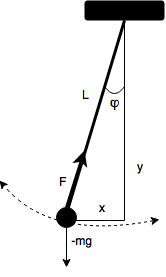
\includegraphics[width=0.2\textwidth]{graphics/pendulum.png}
  \caption{Péndulo plano}
  \label{fig:pendulo}
\end{figure}

Cinco de las ecuaciones del modelo son diferenciales y dos son algebraicas.
Las variables del modelo son $x$, $y$, $v_{x}$, $v_{y}$, $\varphi$,
$\omega$, $F$ y las constantes $L$, $m$, $g$. Hemos reemplazado
la ecuación correspondiente a la ley de Pitagóras por dos ecuaciones
algebraicas sobre las variables $x$ e $y$ respectivamente, las cuales
aún preservan la restricción sobre la longitud del péndulo.

La forma general de un sistema DAE, de la cual el ejemplo anterior
es un caso particular donde $x=\{x,y,v_{x},v_{y},\varphi\}$, $u=\{\}$,
$y=\{$$\omega,F\}$, se puede ver a continuación:

\begin{gather}
F(x(t),\dot{x}(t),u(t),y(t))=0\nonumber \\
G(x(t),u(t),y(t))=0\label{eq:dae}
\end{gather}



\subsection{Simulación de Modelos Continuos}

En la sección anterior vimos como modelar matemáticamente sistemas
dinámicos como ecuaciones diferenciales explícitas (ODEs) o algebraicas
(DAEs). 

Desde el punto de vista del modelador, describir el sistema en forma
de DAE como la ecuación (\ref{eq:dae}) resulta más sencillo (o incluso
la única forma de hacerlo) debido a que partiendo de un modelo de
primeros principios se pueden describir las relaciones constitutivas
de cada componente y las inter-relaciones entre éstos. Por otro lado
la simulación computacional de esta clase de modelos conlleva ciertos
problemas. Primero se deben encontrar condiciones iniciales consistentes
que satisfagan todas las ecuaciones lo cual no es sencillo. Luego,
si el sistema contiene singularidades estructurales, algunas variables
se deberán resolver integrando su derivada y otras derivando la variable.
La derivación numérica no es robusta \citep{CK06} por lo cual sólo
se usa en casos particulares.

En el caso general se prefiere recurrir a métodos de integración para
ODEs ya que éstos siempre integran todas las variables de estado.
Es por ello que los modelos descriptos como DAEs deben ser convertidos
simbólicamente a ODEs. Esta conversión es lo que se conoce como \emph{causalización}
de un modelo y es la cuestión central de este trabajo. Se verá en
detalle en la sección \ref{sub:Transformaci=0000F3n-BLT--}.


\section{El lenguaje Modelica}

Modelica es un lenguaje de modelado (estándar abierto) que permite
la especificación de modelos matemáticos de complejos sistemas naturales
o artificiales con el propósito de posibilitar la simulación computarizada
de sistemas dinámicos que evolucionan con el tiempo. Modelica es también
un lenguaje de programación orientado a objetos y basado en ecuaciones,
pensado para aplicaciones de mucha complejidad que requieren una alta
eficiencia. Las tres características principales son:
\begin{itemize}
\item Modelica está principalmente basado en ecuaciones en lugar de asignaciones.
Esto permite un modelado acausal lo cual facilita la reutilización
de las clases ya que las ecuaciones no especifican una dirección particular
para el flujo de datos. De esta manera una clase Modelica se puede
adaptar a contextos con diferentes flujos de datos.
\item Modelica permite describir y conectar componentes de modelos pertenecientes
a diferentes dominios como eléctricos, mecánicos, termodinámica, hidráulica,
biología, control, etc.
\item Modelica es un lenguaje orientado a objetos con un concepto general
de clase que unifica las ideas de clases, tipos genéricos y subtipos
en un solo lenguaje. Esto facilita la reutilización de componentes
y la evolución de los modelos.
\end{itemize}
Estas son las propiedades que hacen a Modelica un lenguaje potente
y fácil de utilizar, especialmente para modelado y simulación.


\subsection{Modelado matemático orientado a objetos}

Los lenguajes orientados a objetos tradicionales como Smalltalk, Java
o C++, así como también los lenguajes procedurales como Fortran o
C, soportan la programación sobre datos almacenados en memoria. Los
datos almacenados en memoria corresponde a valores de variables y
datos de objetos. El número de objetos usualmente cambia de manera
dinámica. El enfoque de orientación a objetos de Smalltalk enfatiza
el envío de mensajes entre objetos.

El enfoque de Modelica del concepto de orientación a objetos es diferente
ya que Modelica enfatiza el modelado matemático estructurado. La orientación
a objetos es vista como una forma de estructuración para poder manejar
la complejidad de las descripciones de grandes sistemas. Un Modelo
Modelica es principalmente una descripción matemática declarativa.
Las propiedades de los sistemas dinámicos se expresan de manera declarativa
mediante ecuaciones. 

El enfoque declarativo de Modelica sobre la orientación a objetos
se puede resumir en estos puntos:
\begin{itemize}
\item La orientación a objetos es utilizada como un concepto de estructuración,
enfatizando la estructura declarativa y la reutilización de los modelos
matemáticos. Las tres maneras de estructurar son jerarquías, conexiones
entre componentes y herencia.
\item Las propiedades de los modelos dinámicos se expresan de manera declarativa
utilizando ecuaciones.
\item Un objeto es una colección de variables de instancia y ecuaciones
que comparten un conjunto de datos.
\end{itemize}
No obstante
\begin{itemize}
\item La orientación a objetos en el modelado matemático no es considerado
como un intercambio de mensajes entre objetos.
\end{itemize}
La forma declarativa y orientada a objetos de describir sistemas y
su comportamiento que ofrece Modelica es de un nivel más alto de abstracción
del que poseen los lenguajes orientados a objetos tradicionales ya
que ciertos detalles de implementación se omiten. Por ejemplo, no
es necesario escribir código para transportar datos de un objeto a
otro mediante asignaciones. Ese código lo genera automáticamente el
compilador de Modelica a partir de las ecuaciones dadas.

De la misma manera que ocurre en los lenguajes orientados a objetos
ordinarios las clases son plantillas para la creación de objetos.
Tanto variables como ecuaciones pueden ser heredadas entre clases.
También las definiciones de funciones pueden ser heredadas. No obstante,
la especificación de comportamiento se realiza principalmente mediante
ecuaciones en lugar de métodos. También el lenguaje permite escribir
código en forma de algoritmos incluyendo funciones pero esto es una
excepción más que una regla.

Dado que este trabajo se centra en la etapa de causalización y que
en ese momento del proceso de compilación el modelo ya se encuentra
aplanado, es decir solo se compone de variables de tipos básicos y
ecuaciones, no ahondaremos más en las particularidades del sistema
de clases de Modelica. El lector interesado puede consultar en \citep{Fritzson98}.


\subsection{Conceptos básicos}

Un modelo Modelica se construye a partir de clases, también denominadas
modelos. A partir de la definición de una clase es posible crear cualquier
número de objetos que se conocen como instancias de esa clase.

Una clase Modelica contiene elementos, los principales son declaraciones
de variables y ecuaciones; las ecuaciones se agrupan en secciones.
Las variables contienen datos pertenecientes a instancias de una clase.
Las ecuaciones de una clase especifican el comportamiento de las instancias
de dicha clase.

La tradición establece que el primer programa de ejemplo cualquiera
sea el lenguaje de programación es un programa sencillo que simplemente
imprime la cadena de caracteres ``Hello World''. Dado que Modelica
es un lenguaje de modelado basado en ecuaciones, imprimir una cadena
de caracteres no tiene mucho sentido. En su lugar nuestro primer \emph{modelo}
Modelica resuelve una ecuación diferencial trivial.

\[
\dot{x}(t)=-a\times x(t)
\]


La variable $x(t)$ en esta ecuación es una variable dinámica cuyo
valor puede variar con el transcurso del tiempo. La expresión $\dot{x(t)}$
es la derivada temporal de $x$, lo cual en Modelica se representa
como \verb+der(x)+. Dado que todos los programas en Modelica, llamados
modelos, consisten en declaraciones de clases nuestro programa HelloWorld
se declara como una clase:

\begin{lstlisting}[language=Modelica]
class HelloWorld
  Real x(start = 1);
  parameter Real a = 1;
  equation
    der(x) = -a*x;
end HelloWorld;
\end{lstlisting}

El programa contiene la declaración de una clase llamada \verb+HelloWorld+
con una variable, un parámetro y una sola ecuación. El primer atributo
de la clase es la variable \verb+x+, la cual es inicializada al valor
1 en el momento en el que se inicia la simulación. Todas las variables
en Modelica tienen un atributo \verb+start+ con un valor por defecto
el cual usualmente es 0.

El segundo atributo es la variable \verb+a+ la cual es una constante
inicializada a 1 al momento de iniciarse la simulación. Las constantes
de este tipo se declaran utilizando el prefijo \verb+parameter+ para
indicar que permanecen constantes durante la simulación pero que es
un parámetro del modelo que puede tomar un valor distinto para cada
simulación, por ejemplo mediante algún comando del entorno de simulación.

Notar también que las variables poseen un tipo que las antecede cuando
se declaran. En nuestro ejemplo ambas variables poseen el tipo \verb+Real+
esto es valores que pertenecen al conjunto real $\mathbb{R}$.

La única ecuación de nuestro ejemplo especifica que la derivada temporal
de \verb+x+ es igual a la multiplicación de \verb+-a+ por \verb+x+.
En Modelica el signo \verb+=+ siempre significa igualdad, esto es,
define una ecuación y no una asignación como en la mayoría de los
lenguajes de programación. Esto es, podríamos haber descripto la misma
ecuación como:

\begin{lstlisting}
0 = der(x) + a*x;
\end{lstlisting}

donde se ve explícitamente que no es una asignación sino una igualdad.

La derivada temporal de una variable se indica mediante la pseudo-función
\verb+der()+.

Nuestro segundo ejemplo es un poco más complicado, es el modelo matemático
de un péndulo plano (ver figura \ref{fig:pendulo}). Las ecuaciones
del modelo son las presentadas en la sección \ref{sub:Ecuaciones-diferenciales-algebra}.
El código modelica para este sistema es el que se puede ver a continuación.

\begin{lstlisting}[language=Modelica]
class Pendulum "Planar Pendulum"
  parameter Real m=1, g=9.81, L=O.5;
  Real F, phi, omega;
  output Real x(start=O.5) ,y(start=O);
  output Real vx,vy;
  equation
    m*der(vx)=-F*sin(phi);
    m*der(vy)=-F*cos(phi)-m*g;
    der(x)=vx;
    der(y)=vy;
    der(phi)=omega;
    x=L*sin(phi);
    y=-L*cos(phi);
end Pendulum;
\end{lstlisting}

Lo interesante de este modelo es que las dos últimas ecuaciones son
diferentes al resto, son ecuaciones algebraicas, es decir, involucran
solo operaciones algebraicas sobre las variables pero no derivadas.
Las otras cinco ecuaciones son ecuaciones diferenciales, como la ecuación
del ejemplo \verb+HelloWorld+. Los sistemas de ecuaciones que contienen
tanto ecuaciones diferenciales como ecuaciones algebraicas se denominan
sistemas de ecuaciones diferenciales algebraicas (o DAEs por sus siglas
en inglés).

Por último hacemos una observación importante en relación a los modelos
Modelica simulables.
\begin{verse}
\emph{El número de variables debe ser igual al número de ecuaciones}\footnote{\emph{A los fines de la causalización se considera que todas las ecuaciones
son diferentes, incluso si la misma ecuación aparece dos veces.}}\emph{.}
\end{verse}
Esta regla es respetada por los dos modelos que vimos en esta sección
y debe ser respetada por cualquier modelo para ser considerado resoluble.
Por variables nos referimos a algo que pueda variar en el tiempo,
no constantes ni parámetros.


\subsubsection{Variables}

El modelo que vamos a ver a continuación muestra un modelo levemente
más complicado. El cual describe un oscilador de Van der Pol. Notar
que en este ejemplo la palabra clave \verb+model+ se utiliza en lugar
de \verb+class+ casi con el mismo significado.

\begin{lstlisting}[language=Modelica]
model VanDerPol "Van der Pol oscillator model"
  Real x(start = 1) "Descriptive string for x";
  Real y(start = 1) "Descriptive string for y";
  parameter Real alpha = 0.3, beta = 0.3, gamma=0.5, delta=0.7;
  equation
    der(x) = x*(alpha-beta*y);
    der(y) = -y*(gamma-delta*x);
end VanDerPol;
\end{lstlisting}

Este ejemplo contiene la declaración de dos variables dinámicas \verb+x+
e \verb+y+, ambas de tipo \verb+Real+ y con valor inicial 1 al comienzo
de la simulación, lo cual normalmente es al momento t=0.

La palabra clave \verb+parameter+ especifica que la variable permanece
constante durante la simulación, pero que su valor se puede inicializar
antes de una ejecución o entre ejecuciones. Un \verb+parameter+ es
una constante que permite al usuario modificar de manera sencilla
el comportamiento de un modelo, por ejemplo modificando el parámetro
\verb+delta+ el cual influencia considerablemente el comportamiento
del oscilador de Van der Pol. Por el contrario, una constante Modelica
declarada con el prefijo \verb+constant+ nunca cambia y puede ser
sustituida por su valor en los lugares donde ocurra.

Por último hay una sección para ecuaciones declarada con la palabra
clave \verb+equation+, conteniendo dos ecuaciones mutuamente dependientes
que definen la dinámica del modelo.


\subsection{Arreglos}

Un arreglo es una colección de variables todas del mismo tipo. Los
elementos de un arreglo se acceden por medio de índices enteros cuyos
valores van desde 1 hasta el tamaño de la respectiva dimensión. Una
variable de tipo arreglo se puede declarar agregando dimensiones entre
corchetes después del nombre de una clase, como en Java, o después
del nombre de una variable, como en C. Por ejemplo:

\begin{lstlisting}[language=Modelica]
  Real[3] positionvector = {1,2,3};
  Real[3,3] identitymatrix = {{1,0,0}, {0,1,0}, {0,0,1}};
  Real[10,20,30] arr3d;
\end{lstlisting}

Esto declara un vector, una matriz de transformación y un arreglo
de tres dimensión 10, 20 y 30 correspondientemente.

Más detalles sobre arreglos en Modelica se pueden encontrar en \citep{Fritzson:2003:POM:966262}.


\subsection{Ecuaciones}

Como ya hemos mencionado, Modelica es principalmente un lenguaje basando
en ecuaciones a diferencia de los lenguajes de programación ordinarios
donde proliferan las asignaciones. Las ecuaciones son más flexibles
que las asignaciones dado que no determinan un flujo de datos u orden
de ejecución particular. Esta es la clave de las capacidades de modelado
de sistemas físicos y del potencial de reutilización de las clases
Modelica.

Pensar en términos de ecuaciones es poco usual para la mayoría de
los programadores. En Modelica tienen lugar las siguientes afirmaciones:
\begin{itemize}
\item Lo que en lenguajes convencionales se define con asignaciones en general
en Modelica se define con ecuaciones.
\item La asignación de valores a atributos se representa como ecuaciones.
\item Las conexiones entre objetos generan ecuaciones.
\end{itemize}
Las ecuaciones son más poderosas que las asignaciones. Por ejemplo,
consideremos la ecuación característica de una resistencia:

\begin{align*}
R\times i & =v
\end{align*}


donde $R$ es el valor de la resistencia.

Esta ecuación puede ser utilizada de tres maneras correspondientes
a tres asignaciones posibles: calcular la corriente a partir del voltaje
y de la resistencia, calcular el voltaje a partir de la resistencia
y de la corriente o calcular la resistencia a partir del voltaje y
de la corriente. A continuación vemos las tres posibles asignaciones:

\begin{align*}
i & :=\frac{v}{R}\\
v & :=R\times i\\
R & :=\frac{v}{i}
\end{align*}


Las ecuaciones en Modelica se pueden clasificar informalmente en cuatro
grupos dependiendo en el contexto sintáctico en el que aparezcan:
\begin{itemize}
\item Ecuaciones normales, las cuales aparecen en la sección \verb+equation+.
\item Ecuaciones que aparecen en la sección de declaraciones y forman parte
de la declaración de una variable o constante.
\item Ecuaciones como modificadores las cuales se utilizan para modificar
atributos.
\item Ecuación de inicialización las cuales se especifican en la sección
\verb+initial equation+ o como para indicar el valor del atributo
\verb+start+. Estas ecuaciones se utilizan para resolver el problema
de inicialización al momento de inicio de la simulación.
\end{itemize}
Como ya hemos visto en los ejemplos anteriores las ecuaciones normales
aparecen en las secciones delimitadas por la palabra clave \verb+equation+
y por alguna otra palabra clave permitida:

\begin{lstlisting}[language=Modelica]
	equation
		...
		<equations>
		...
	<some other allowed keyword> 
\end{lstlisting}

La ecuación de la resistencia que mostramos más arriba es un ejemplo
de una ecuación que puede ser ubicada en una sección \verb+equation+.
Las ecuaciones que aparecen en la sección de declaraciones generalmente
se utilizan como parte de la declaración de constantes paramétricas
o fijas, por ejemplo:

\begin{lstlisting}[language=Modelica]
	constant Integer one = 1;
	parameter Real mass = 22.5; 
\end{lstlisting}

La veracidad de una ecuación se mantiene siempre, lo que significa
que la masa en el ejemplo anterior nunca varia durante la simulación.
También es posible especificar una ecuación en la declaración de una
variable común, por ejemplo:

\begin{lstlisting}[language=Modelica]
	Real speed = 72.4; 
\end{lstlisting}

Sin embargo esto no tiene mucho sentido ya que va a restringir la
variable a que tenga el mismo valor durante toda la ejecución haciendo
que se comporte como una constante. De esta manera se puede notar
que la utilización de una ecuación en la declaración de una variable
es bastante diferente de la inicialización de una variable en otros
lenguajes.

Las asignaciones de valores a atributos se realizan utilizando ecuaciones
como modificadores. Por ejemplo, si necesitamos especificar un valor
inicial para una variable lo que hacemos es definir una ecuación para
el atributo \verb+start+ de la variable:

\begin{lstlisting}[language=Modelica]
	Real speed(start=72.4); 
\end{lstlisting}

Cabe destacar que la causalización se aplica sobre las ecuaciones
normales, es decir las declaradas en las secciones \verb+equation+.


\subsubsection{Ecuaciones con Estructuras Repetitivas}

A veces surge la necesidad de expresar convenientemente conjuntos
de ecuaciones con estructuras que se repiten. Para estos casos Modelica
ofrece un tipo particular de ecuación denominado loop equation. Notar
que esto no es un bucle en el sentido algorítmico de la palabra sino
que es una forma abreviada de expresar un conjunto de ecuaciones.

Por ejemplo, consideremos una ecuación para una expresión polinomial:

$\begin{aligned}y & = & a[1]+a[2]\times x+a[3]\times x^{2}+\ldots+a[n+1]\times x^{n}\end{aligned}
$

La ecuación polinomial se puede expresar como un conjunto de ecuaciones
con la misma estructura más una ecuación adicional donde $y$ es igual
al producto escalar de los vectores a y xpowers, ambos de longitud
n+1:

\begin{lstlisting}[language=Modelica]
  xpowers[1] = 1;
  xpowers[2] = xpowers[1]*x;
  xpowers[3] = xpowers[2]*x;
  ...
  xpowers[n+1] = xpowers[n]*x;
  y = a * xpowers;
\end{lstlisting}

El conjunto de ecuaciones sobre las variables \verb+xpowers+ se pueden
expresar de manera más conveniente utilizando la notación \verb+for+:

\begin{lstlisting}[language=Modelica]
  for i in 1:n loop
    xpowers[i+1] = xpowers[i]*x;
  end for;
\end{lstlisting}


\section{Manipulación simbólica de modelos Modelica}

Vamos a comenzar la sección detallando brevemente los pasos necesarios
para traducir y simular un modelo Modelica. Luego profundizaremos
en las técnicas de manipulación simbólica utilizadas para convertir
los modelos DAE en modelos ODE ordenados.


\subsection{\label{sec:Implementaci=0000F3n-y-ejecuci=0000F3n}Compilación y
Simulación de modelos Modelica}

El primer paso del proceso de compilación consisten en un análisis
sintáctico del código fuente Modelica del cual se obtiene un árbol
sintáctico abstracto. Luego esta representación se analiza gramaticalmente,
se realiza la verificación de tipos, las clases se heredan y expanden,
se realizan las modificaciones e instanciaciones correspondientes,
las ecuaciones \verb+connect+ se convierten en ecuaciones comunes,
etc. El resultado de este proceso de análisis y traducción es un conjunto
plano de ecuaciones, constantes, variables y funciones. No queda ningún
rastro de la estructura de objetos.

Después del proceso de aplanado todas las ecuaciones se ordenan topológicamente
de acuerdo a las dependencias del flujo de datos entre ellas. En el
caso de ecuaciones diferenciales algebraicas, no solo se realiza un
ordenamiento, sino que también es necesario manipular las ecuaciones
para convertir la matriz de coeficientes a forma triangular inferior
de a bloques, lo que usualmente se denomina transformación BLT por
sus siglas en ingles \citep{Fritzson98}. Luego un módulo de optimización
compuesto por algoritmos de simplificación algebraica, métodos de
reducción de índices, etc., elimina la mayoría de las ecuaciones dejando
solo un conjunto mínimo que eventualmente va a ser resuelto numéricamente.
Por ejemplo, si dos variables son sintácticamente equivalentes solo
se conserva una.

La etapa siguiente consiste en convertir las ecuaciones independientes
resultantes en asignaciones. Esto es posible dado que las ecuaciones
fueron ordenadas y se determinó una secuencia de ejecución para la
evaluación de las ecuaciones. Si aparece un conjunto de ecuaciones
fuertemente conectadas (un bucle algebraico) se realizan transformaciones
simbólicas que ejecutan una serie de transformaciones algebraicas
para simplificar las dependencias entre las variables. En ciertos
casos se puede resolver el sistema de ecuaciones que representa el
lazo si este posee solución simbólica.

Finalmente se genera código en algún lenguaje de programación convencional,
usualmente C, y se lo enlaza con algún método de integración numérica
el cual es el encargado de resolver el sistema de ecuaciones resultante,
sistema que ya a sido drásticamente reducido.

En la figura \ref{fig:compilacion_Modelica} se pueden ver las distintas
etapas del proceso de traducción y ejecución.

\begin{figure}[H]
  \centering
  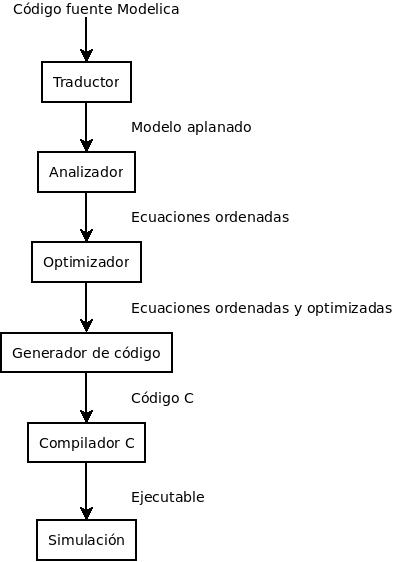
\includegraphics[width=0.3\textwidth]{graphics/EtapasCompilacion.jpg}
  \caption{Etapas del proceso de compilación y ejecución de Modelica.}
  \label{fig:compilacion_Modelica}
\end{figure}


\subsection{Simplificación Simbólica de Modelos Modelica}

Como mencionamos previamente luego del proceso de aplanado de la estructura
de objetos lo que se obtiene es un sistema de ecuaciones diferenciales
algebraicas. Simular un modelo Modelica en general consiste en resolver
sistemas de ese tipo. Esta tarea no es trivial por varias razones:
\begin{itemize}
\item Las ecuaciones no solo poseen incógnitas de tipo \verb+Real+ sino
también \verb+Boolean+, \verb+Integer+ y \verb+enumeration+.
\item La naturaleza orientada a objetos de los modelos Modelica, los cuales
usualmente consisten de muchos componentes conectados, resulta después
del aplanado en sistemas DAE bastante ralos (una matriz asociada con
muchos ceros) \citep{elmqvist2005}.
\item Las orientación a objetos da lugar a que los usuarios escriban modelos
muy grandes, incluso modelos con varias cientos de miles de ecuaciones
y variables. Modelos tan grandes plantean demandas especiales sobre
las técnicas de solución.
\end{itemize}
Muchas de estas dificultades pueden ser resueltas manipulando simbólicamente
el sistema de ecuaciones antes de aplicar un método de integración
numérico. En la sección \ref{sec:Implementaci=0000F3n-y-ejecuci=0000F3n}
mencionamos el método de realizar una partición BLT, o ordenamiento
topológico, del sistema de ecuaciones utilizando el algoritmo de Tarjan
\citep{Tarjan72}. Este algoritmo encuentra los componentes fuertemente
conexos conteniendo ecuaciones mutuamente dependientes, i.e bucles
algebraicos. El particionado del sistema de ecuaciones posibilita
una solución más eficiente reduciendo la cantidad de variables que
tienen que ser manejadas por el método de integración en cada subsistema
de ecuaciones. 

Algunos de los subsistemas de ecuaciones simultaneas encontrados por
el particionado BLT son lineales y pueden ser resueltos por algoritmos
de álgebra estándar de sistemas de ecuaciones lineales. Otros sistemas
resultan ser no lineales. Una técnica denominada \textit{tearing}
puede reducir aún más el tamaño y contribuir a mejorar la eficiencia
cuando se resuelven este tipo de sistemas de ecuaciones no lineales
\citep{CK06}. La técnica de tearing permite resolver de manera secuencial
pero iterativamente las ecuaciones de un subsistema eligiendo en cada
iteración la ``tearing variable'' y comenzando con un primera aproximación
del valor de la variable. La convergencia de este proceso no está
garantida, sin embargo en la mayoría de los casos ocurre.

La necesidad de diferenciar numéricamente utilizando métodos de integración
númericos de DAEs puede ser reducida o eliminada empleando el algoritmo
de Pantelides para la \textit{reducción de índice }el cual transforma
simbólicamente el sistema de ecuaciones a una forma de menor índice.
El sistema de ecuaciones resultantes con índice no mayor a 1 puede
ser resuelto por algoritmos de integración numérica como DASSL \citep{DASSL}
o DOPRI \citep{DP80} y incluso en algunos casos utilizando simples
métodos de resolución de ODEs como Euler \citep{CK06}.

Descripciones de la técnica de tearing y del algoritmo de Pantelides
se pueden encontrar en los siguientes libros \citep{Fritzson:2003:POM:966262,CK06}.
En la sección siguiente vamos a explicar en qué consiste la transformación
o particionado BLT del sistema de ecuaciones también denominado proceso
de causalización de ecuaciones.


\section{\label{sub:Transformaci=0000F3n-BLT--}Causalización - Transformación
BLT}

Los sistemas de ecuaciones diferenciales algebraicas resultantes de
aplanar la estructura de objetos de un modelo Modelica por lo general
son grandes, ralos (una matriz de incidencia asociada con muchos ceros)
y no lineales \citep{elmqvist2005}.

Permutando las ecuaciones y las variables es posible transformar el
sistema de ecuaciones, o mejor dicho la matriz asociada, a una forma
triangular inferior de a bloques (o BLT por sus siglas en inglés).
Una vez llevado a esta forma BLT el sistema puede ser resuelto secuencialmente.
Vamos a explicar la idea utilizando un ejemplo simple el cual consiste
de 3 ecuaciones no lineales.
\begin{gather}
h_{1}(z_{1},z_{3})=0\nonumber \\
h_{2}(z_{2})=0\nonumber \\
h_{3}(z_{1},z_{2})=0\label{eq:ej_transformacion_blt_sis}
\end{gather}


\begin{gather}
S_{1}=\begin{array}{c}
\begin{array}{ccc}
z_{1} & z_{2} & z_{3}\end{array}\\
\left[\begin{array}{ccc}
1 & 0 & 1\\
0 & 1 & 0\\
1 & 1 & 0
\end{array}\right]
\end{array}\label{eq:ej_transformacion_blt_matriz}
\end{gather}


La matriz $S_{1}$describe la estructura del sistema de ecuaciones.
La entrada S$_{ij}$ es 1 si la variable i aparece en la ecuación
j y 0 en caso contrario. Permutando las ecuaciones y las variables
este conjunto de ecuaciones puede ser llevado a la forma BLT:

\begin{gather}
h_{2}(z_{2})=0\nonumber \\
h_{3}(z_{1},z_{2})=0\label{eq:ej_transformacion_blt_sis_2}\\
h_{1}(z_{1},z_{3})=0\nonumber 
\end{gather}


\begin{gather}
S_{2}=\begin{array}{c}
\begin{array}{ccc}
z_{2} & z_{1} & z_{3}\end{array}\\
\left[\begin{array}{ccc}
1 & 0 & 0\\
1 & 1 & 0\\
0 & 1 & 1
\end{array}\right]
\end{array}\label{eq:ej_tranformacion_blt_matriz_2}
\end{gather}


Este proceso se denomina particionado del conjunto de ecuaciones.
La forma triangular inferior estricta de la matriz asociada al sistema
permite ver el hecho de que las ecuaciones no lineales pueden ser
resueltas una por vez de manera secuencial. Comenzamos resolviendo
$h_{2}$ para la variable $z_{2}$, luego, conociendo $z_{2}$ podemos
resolver $h3$ para $z_{1}$ y finalmente podemos determinar $z_{3}$
a partir de $h_{1}$ ya conociendo $z_{2}$ y $z_{1}$. Si la variable
a resolver aparece linealmente en una ecuación, la variable puede
ser despejada mediante manipulación simbólica. En caso contrario se
requiere una iteración local de Newton.

En general no es posible transformar la matriz asociada a la forma
triangular inferior estricta. Sin embargo existen algoritmos eficientes
para convertir la matriz a una forma triangular inferior de a bloques,
esto es una forma cuasi-triangular inferior en donde a lo largo de
la diagonal aparecen bloques de dimensión $\geqq1$. Un ejemplo de
matriz triangular inferior de a bloques se puede ver en la figura
\ref{fig:post_Tarjan} de la sección \ref{sub:Aplicacion-Tarjan-Marco-Teorico}.
Esta no es una matriz triangular inferior estricta ya que la celda
($f{}_{3}$, $z{}_{5}$), la cual posee un valor distinto de cero,
se encuentra por encima de la diagonal. No obstante, dicha celda pertece
a una submatriz o bloque de $2\times2$. Entonces considerando al
resto de los elementos de la diagonal como bloques de $1\times1$
podemos decir que la matriz es triangular inferior de a bloques.

Los algoritmos que permiten transformar una matriz en la forma BLT
garantizan que las dimensiones de los bloques son del menor tamaño
posible. Es decir no se pueden obtener bloques más pequeños mediante
la permutación de variables y ecuaciones. Los bloques de tamaño $>1$
corresponden a sistemas de ecuaciones que tienen que ser resueltos
simultáneamente. A estos sub-sistemas de ecuaciones mutuamente dependientes
se los denomina lazos algebraicos. Finalmente podemos concluir que
los algoritmos de particionado encuentra lazos algebraicos de dimensiones
mínimas.


\subsection{\label{sub:Algoritmos-de-grafos}Algoritmos de grafos para obtener
la transformación BLT}

En el artículo \citep{Duff:1978:ITA:355780.355785} se demuestra que
la forma más eficiente de calcular la transformación BLT de una matriz
es aplicando el algoritmo de Tarjan \citep{Tarjan72}. Este es un
algoritmo perteneciente a la teoría de grafos, el cual permite encontrar
los componentes fuertemente conexos en un grafo dirigido.

Dada una matriz $S$, para poder aplicar el algoritmo de Tarjan y
obtener una transformación BLT, es necesario construir un grafo dirigido
compuesto por un conjunto de n nodos, etiquetados $1,2,3,\ldots,n$
y un conjunto de aristas $(i,j)$ cada una de las cuales es un par
ordenado de nodos correspondiente a una entrada $S_{ij}$ distinta
de cero y ubicada fuera de la diagonal. Realizar una permutación de
la matriz $S$ se corresponde con re-etiquetar los nodos del grafo.

Se dice que un subgrafo es fuertemente conexo si existe un camino
desde cualquiera de sus nodos hacia cualquier otro nodo y que es un
componente fuertemente conexo si no puede ser agrandado a otro subgrafo
fuertemente conexo agregando nodos y las aristas asociadas. Claramente,
cada nodo puede pertenecer solo a un componente fuertemente conexo
(que puede componerse de un solo nodo) por lo tanto los componentes
fuertemente conexos determinan una partición del grafo. Debe haber
al menos un componente fuertemente conexo tal que no exista camino
de ninguno de sus nodos hacia algún nodo de otro componente. Denominemos
$C_{1}$a este componente. Los otros componentes fuertemente conexos
$C_{2},C_{3},\ldots,C_{k}$ pueden ser elegidos aplicando el mismo
criterio de manera tal que no exista ningún camino de un nodo en un
componente fuertemente conexo hacia un nodo de un componente fuertemente
conexo que aparezca después en la secuencia.

Si estos componentes fuertemente conexos son identificados en el orden
mostrado en el párrafo anterior, y los nodos de $C_{1}$son numerados
antes de los nodos de $C_{2}$, y así sucesivamente, entonces la matriz
asociada es triangular de a bloques donde los bloques se corresponden
con los componentes fuertemente conexos del grafo. Además, dado que
el subgrafo asociado con cada submatriz de la diagonal en la forma
de a bloques es fuertemente conexo, es evidente que los bloques no
pueden ser permutados a la forma BLT.

En el artículo\citep{Duff:1978:ITA:355780.355785} Duff presenta dos
algoritmos que exhiben esta propiedad en donde los componentes fuertemente
conexos son identificados en un orden tal que los nodos de cada componente
pueden poseer caminos que conducen a nodos de componentes previos
pero nunca a nodos de componentes posteriores. Estos algoritmos son
el de Sargent and Westerber \citep{sargent1964speed} y el de Tarjan.
Mientras el algoritmo de Sargent and Westerber presenta una complejidad
temporal (en función de la cantidad de variables) en el peor caso
de $O(n^{2})$ el algoritmo de Tarjan se ejecuta en $O(n)+O(\tau)$
donde $\tau$ es la cantidad de entradas de la matriz que no pertenecen
a la diagonal y son diferentes de 0.


\subsection{Algoritmo de Tarjan para encontrar los componentes fuertemente conexos
de un grafo}

El algoritmo de Tarjan recibe como entrada un grafo dirigido y produce
una partición de los vértices del grafo en componentes fuertemente
conexos. Cada vértice del grafo aparece en un solo componente fuertemente
conexo. Un vértice que no pertenece a ningún ciclo constituye por
si solo un componente fuertemente conexo.

La idea básica del algoritmo es la siguiente: comenzando por cualquier
nodo se realiza una búsqueda en profundidad (y subsiguientes búsquedas
se realizan sobre cualquier nodo que no haya sido visitado aún). Como
es usual en las búsquedas en profundidad, el proceso de búsqueda visita
cada nodo una sola vez y rechaza visitar un nodo que ya fue explorado.
En consecuencia la colección de árboles de búsqueda es un bosque recubridor
del grafo. Los componentes fuertemente conexos se van a obtener a
partir de algunos subárboles del bosque recubridor. Las raíces de
estos árboles serán las raíces de los componentes fuertemente conexos.
Cualquier nodo de un componente fuertemente conexo puede ser el nodo
raíz siempre y cuando haya sido el primer nodo en ser descubierto
para ese componente.

Los nodos se van almacenando en una pila en el orden en el que se
van encontrando. Cuando el proceso de búsqueda en profundidad recursivamente
explora un nodo v y sus descendientes, dichos nodos no necesariamente
son retirados (popped) de la pila antes de que la llamada recursiva
termine. La propiedad invariante fundamental es que un nodo permanece
en la pila después de ser explorado si y solo si posee un camino (path)
hacia un nodo ingresado previamente en la pila.

Al final de la llamada que explora el nodo v y sus descendientes sabemos
si este posee algún camino hacia un nodo ingresado previamente en
la pila. De ser así la llamada retorna dejando el vértice v en la
pila para preservar el invariante. En caso contrario v debe ser la
raíz de su componente fuertemente conexo el cual consiste en v más
cualquier nodo colocado posteriormente. El componente identificado
se retira de la pila.

A cada nodo v se le asigna un entero único \verb+v.index+ el cual
numera los nodos de manera consecutiva en el orden en el que son descubiertos.
Además para cada nodo también se mantiene un valor denominado \verb+v.lowlink+
el cual representa el menor índice asociado a un nodo accesible desde
v, incluido el mismo v. De esta manera v debe ser mantenido en la
pila si \verb+v.lowlink < v.index+, y v debe ser removido de la pila
si \verb+v.lowlink == v.index+. El valor \verb+v.lowlink+ es calculado
durante la búsqueda en profundidad originada en v. 

A continuación vemos el algoritmo en pseudo-código:

\begin{lstlisting}
algorithm Tarjan is
  input: graph G = (V, E)
  output: set of strongly connected components (sets of vertices) 
 
  index := 0 
  S := empty

  for each v in V do
    if (v.index is undefined) then
      strongconnect(v)
    end if
  end for

  function strongconnect(v)
    // Set the depth index for v to the smallest unused index
    v.index := index
    v.lowlink := index
    index := index + 1
    S.push(v)
    v.onStack := true

    // Consider successors of v
    for each (v, w) in E do
      if (w.index is undefined) then
        // Successor w has not yet been visited;
        strongconnect(w)
        v.lowlink  := min(v.lowlink, w.lowlink)
      else if (w.onStack) then
        // Successor w is in stack S and hence in the current SCC
        v.lowlink  := min(v.lowlink, w.index)
      end if
    end for
    
    // If v is a root node, pop the stack and generate an SCC
    if (v.lowlink = v.index) then
      start a new strongly connected component
      repeat
        w := S.pop()
        w.onStack := false
        add w to current strongly connected component
      while (w != v)
      output the current strongly connected component
    end if
  end function
\end{lstlisting}

Vamos a finalizar la sección aplicando el algoritmo sobre el grafo
de la figura \ref{fig:tarjan_step_0}. Entre las figuras \ref{fig:tarjan_step_1}
y \ref{fig:tarjan_step_4} se puede ver la evolución del algoritmo.
En cada una de las figuras se destaco con linea de trazo continuo
el camino que condujo a la identificación de un componente fuertemente
conexo. Junto a cada nodo se incluyo el valor de las variables \verb+index+
y \verb+lowlink+. También se incluyo junto a cada figura el estado
de la pila en el momento previo a la identificación del componente.

\begin{figure}[H]
    \begin{subfigure}[b]{0.3\textwidth}
    \includegraphics[width=0.8\textwidth]{graphics/revision/tarjan_step_0.png}
    \caption{\label{fig:tarjan_step_0}}
  \end{subfigure}
  \begin{subfigure}[b]{0.3\textwidth}
    \includegraphics[width=0.8\textwidth]{graphics/revision/tarjan_step_1.png}
    \caption{\label{fig:tarjan_step_1}}
  \end{subfigure}
  \begin{subfigure}[b]{0.3\textwidth}
    \includegraphics[width=0.8\textwidth]{graphics/revision/tarjan_step_2.png}
    \caption{\label{fig:tarjan_step_2}}
  \end{subfigure}
  \begin{subfigure}[b]{0.3\textwidth}
    \includegraphics[width=0.8\textwidth]{graphics/revision/tarjan_step_3.png}
    \caption{\label{fig:tarjan_step_3}}
  \end{subfigure}
  \begin{subfigure}[b]{0.3\textwidth}
    \includegraphics[width=0.8\textwidth]{graphics/revision/tarjan_step_4.png}
    \caption{\label{fig:tarjan_step_4}}
  \end{subfigure}
  \caption{\label{fig:tarjan_step_by_step}}
\end{figure}


\subsection{\label{sub:Aplicacion-Tarjan-Marco-Teorico}Aplicación del algoritmo
de Tarjan para obtener la forma BLT}

En esta sección vamos explicar cómo aplica el algorítmo de Tarjan
en la transformación a la forma triangular inferior de a bloques de
la matriz asociada a un sistema de ecuaciones algebraicas.

Para explicar el algoritmo vamos a utilizar el sistema de ecuaciones
diferenciales algebraicas que aparece en la figura \ref{fig:pre_Tarjan}
junto con su matriz de coeficientes asociada. La matriz de coeficientes
posee una fila por cada ecuación y una columna por cada incógnita.
Una entrada (i,j) de la matriz toma el valor 1 si la variable j ocurre
en la ecuación i. En caso contrario la entrada de la matriz es 0.

\begin{figure}[H]
  \centering
  \begin{align*}
    f_1(z_3,z_4) &= 0 \\
    f_2(z_2) &= 0 \\
    f_3(z_2,z_3,z_5) &= 0 \\
    f_4(z_1,z_2) &= 0 \\
    f_5(z_1,z_3,z_5) &= 0 \\
  \end{align*}
  \bordermatrix{
       & z_1 & z_2 & z_3 & z_4 & z_5 \cr
   f_1 & 0   & 0   & 1   & 1   & 0 \cr
   f_2 & 0   & 1   & 0   & 0   & 0 \cr
   f_3 & 0   & 1   & 1   & 0   & 1 \cr
   f_4 & 1   & 1   & 0   & 0   & 0 \cr
   f_5 & 1   & 0   & 1   & 0   & 1 \cr
  }
  \caption{Sistema de ecuaciones junto con la matriz de adjacencia asociada.\label{fig:pre_Tarjan}}
\end{figure}

Tal como explicamos en la sección \ref{sub:Algoritmos-de-grafos},
para poder obtener la transformación BLT de una matriz, necesitamos
construir un grafo dirigido a partir de la misma y aplicar el algoritmo
de Tarjan sobre ese grafo. En el caso de la matriz de coeficientes
asociada a un sistema de ecuaciones diferenciales el grafo que se
obtiene es un grafo bipartito no dirigido. Por lo tanto es necesario
generar a partir de este un grafo dirigido sobre el cual poder aplicar
el algoritmo de Tarjan. En la figura \ref{fig:grafo_pre_Tarjan} se
puede ver el grafo bipartito asociado a la matriz de coeficientes
del ejemplo.

Notar que en la figura \ref{fig:grafo_pre_Tarjan} hemos destacada
un conjunto de vértices y algunas de sus aristas adjacentes. Estos
vértices forman un componente fuertemente conexo. Dicho componente
se corresponde con un lazo algebraico del sistema de ecuaciones compuesto
por las ecuaciones $f_{3}$ y $f_{5}$. Más adelante, en la figura
\ref{fig:system_post_Tarjan} se puede ver como, después de aplicar
el algoritmo de Tarjan, el lazo algebraico formado por las ecuaciones
$f_{3}$ y $f_{5}$ queda correctamente ordenado después de las ecuaciones
$f_{2}$ y $f_{4}$ de la cuales depende.

\begin{figure}[H]
   \centering
   \includegraphics[width=0.3\textwidth]{graphics/revision/bipartito_original.png}
   \caption{Grafo bipartito correspondiente a la forma inicial del sistema de eucaciones.}
   \label{fig:grafo_pre_Tarjan}
\end{figure}

A partir del grafo bipartito se puede construir el grafo dirigido
siguiendo los pasos que describimos a continuación.
\begin{enumerate}
\item Calculamos un emparejamiento\footnote{Del termino ingles ``matching''.}
máximo sobre el grafo original.
\item Para cada $v{}_{e}$ perteneciente al conjunto de vértices del grafo
original asociados a ecuaciones creamos un vértice $v_{e}^{d}$ en
el nuevo grafo dirigido.
\item Para cada par de aristas del grafo original ($v{}_{e1}$, $v{}_{i}$)
y ($v{}_{e2}$, $v{}_{i}$), dentro y fuera del emparejamiento respectivamente,
trazamos una arista en el grafo dirigido. Esta arista tendra como
vértice de origen a $v{}_{e2}^{d}$ y como vértice destino a $v{}_{e1}^{d}$.
\end{enumerate}
En la figura \ref{fig:matching} se puede ver el matching para el
grafo bipartito \ref{fig:grafo_pre_Tarjan}. El grafo dirigido, resultante
de aplicar los pasos 2 y 3, se puede ver en la figura \ref{fig:colapsado}.
Finalmente en la figura \ref{fig:strong_components} se pueden ver
los componentes fuertemente conexos en los que fue particionado el
grafo luego de la aplicación del algoritmo de Tarjan. En la figura
también se aprecia el orden en el que se identificaron los componentes.
El detalle del proceso de identificación de cada uno de los componentes
fuertemente conexos se puede ver en la figura \ref{fig:tarjan_step_by_step}.

\begin{figure}[H]
  \centering
  \begin{subfigure}[b]{0.3\textwidth}
    \includegraphics[width=0.8\textwidth]{graphics/revision/bipartito_matching.png}
    \caption{\label{fig:matching}}
  \end{subfigure}
  \begin{subfigure}[b]{0.3\textwidth}
    \centering
    \includegraphics[width=1\textwidth]{graphics/revision/dirigido.png}
    \caption{\label{fig:colapsado}}
  \end{subfigure}
  \begin{subfigure}[b]{0.4\textwidth}
    \centering
    \includegraphics[width=1\textwidth]{graphics/revision/dirigido_componentes.png}
    \caption{\label{fig:strong_components}}
  \end{subfigure}
\caption{Aplicación del algoritmo de Tarjan\label{fig:aplicacion_tarjan}}
\end{figure}

A partir del orden de los componentes fuertemente conexos que arroja
el algoritmo de Tarjan podemos reordenar las columnas y filas de la
matriz de coeficientes del sistema de ecuaciones. Es decir la fila
correspondiente a la ecuación $f{}_{2}$ y la columna correspondiente
a la variable $z{}_{2}$ se ubican en la primer posición, luego la
fila correspondiente a $f{}_{4}$ y la columna correspondiente a $z{}_{1}$
ocupan la segunda posición y así sucesivamente. La figura \ref{fig:matrix_post_Tarjan}
muestra la matriz de coeficientes resultante, la cual ha sido transformada
a la forma triangular inferior de a bloques. El lazo algebraico destacado
en la figura \ref{fig:grafo_pre_Tarjan} constituye un bloque de tamaño
2 en la diagonal de la matriz de coeficientes. El sistema de ecuaciones
ordenado a partir del orden de los componentes fuertemente conexos
determinado por el algoritmo de Tarjan, se puede ver en la figura
\ref{fig:system_post_Tarjan}.

\begin{figure}[H]
  \centering
  \hspace*{\fill} 
  \begin{subfigure}[b]{0.3\textwidth}
  \bordermatrix{
       & z_2 & z_1 & z_3 & z_5 & z_4 \cr
   f_2 & \mathbf{1}   & 0   & 0   & 0   & 0 \cr
   f_4 & 1   & \mathbf{1}   & 0   & 0   & 0 \cr
   f_3 & 1   & 0   & \mathbf{1}   & \mathbf{1}   & 0 \cr
   f_5 & 0   & 1   & \mathbf{1}   & \mathbf{1}   & 0 \cr
   f_1 & 0   & 0   & 1   & 0   & \mathbf{1} \cr
  }
  \subcaption{Matriz de coeficientes reordenada en forma triangular inferior de a bloques\label{fig:matrix_post_Tarjan}}
  \end{subfigure}
  \hfill
  \begin{subfigure}[b]{0.3\textwidth}
  \begin{align*}
    f_2(z_2) &= 0 \\
    f_4(z_1,z_2) &= 0 \\
    \mathbf{f_3(z_2,z_3,z_5)} &= \mathbf{0} \\ 
    \mathbf{f_5(z_1,z_3,z_5)} &= \mathbf{0} \\
    f_1(z_3,z_4) &= 0 \\
  \end{align*}
  \subcaption{Sistema de ecuaciones reordenado según las dependencias entre las ecuaciones.\label{fig:system_post_Tarjan}}
  \end{subfigure}
  \hspace*{\fill}
  \caption{\label{fig:post_Tarjan}}
\end{figure}


\chapter{\label{chap:Visi=0000F3n-general-del}Visión general del Compilador}

El compilador ModelicaCC \citep{lsmodelica,ModelicaCC} (Modelica
C Compiler) se desarrolló como un conjunto de componentes independientes,
cada uno de los cuales implementa una etapa diferente del proceso
de compilación de un modelo Modelica. En este capítulo vamos a introducir
los diferentes componentes que conforman el compilador Modelica explicando
el rol de cada uno y cómo se componen para lograr la compilación de
un modelo Modelica.


\section{Introducción}

La compilación de un modelo Modelica es el proceso mediante el cual
se transforma un modelo de alto nivel, el cual puede contener clases
y ecuaciones acausales, en un modelo plano, sin clases, y donde las
ecuciones se encuentran ordenadas o causalizadas. Un modelo plano
con las ecuaciones ordenadas de manera tal que para cada ecuación
las variables del lado derecho se pueden considerar conocidas es un
modelo apropiado para la generación de código C (o de cualquier otro
lenguaje similar) y su posterior simulación.

\begin{figure}[h]
  \centering
  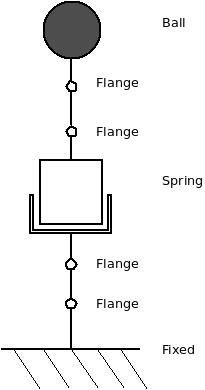
\includegraphics[width=0.3\textwidth]{graphics/BouncingBall.png}
  \caption{Bouncing Ball}
  \label{fig:bouncing_ball}
\end{figure}

Como ya mencionamos en la sección \ref{sec:Implementaci=0000F3n-y-ejecuci=0000F3n}
el proceso de compilación consiste en primer lugar en un análisis
sintáctico y semántico. Luego se realiza un aplanado del modelo obteniendo
un modelo equivalente sin clases y con las ecuaciones \verb+connect+
convertidas en ecuaciones comunes. Luego las ecuaciones acausales
del modelo aplanado se causalizan ordenándolas topológicamente de
acuerdo a las dependencias del flujo de datos entre ellas.

El proceso de análisis sintáctico, semántico y aplanado es responsabilidad
de un componente denominado flatter. La siguiente etapa consiste en
reescribir el modelo utilizando un subconjunto del lenguaje Modelica
denominado μModelica. Finalmente tenemos la causalización del conjunto
de ecuaciones del modelo, la cual es tarea de un componente denominado
causalize. En las siguientes secciones vamos a describir con más detalle
cada una de estos componentes.

Para ayudar a comprender las transformaciones que realizan sobre un
modelo Modelica los diferentes componentes vamos a utilizar un ejemplo.
El ejemplo es el modelo orientado a objetos de un sistema mecánico.
El sistema es una pelota que rebota contra el suelo.

En la figura \ref{fig:bouncing_ball} se pueden ver gráficamente el
modelo. Nuestro modelo contempla la situación de la pelota en contacto
con el suelo y en el aire. Cuando está en el aire el modelo de la
misma es el de una masa puntual sobre la cual sólo actúa la fuerza
de la gravedad y al estar en contacto con el piso, el modelo consiste
en una masa puntual vinculada con el piso a través de un resorte y
un amortiguador dispuestos en paralelo. Ni el resorte ni el amortiguador
existen en la realidad pero son necesarios para representar la capacidad
de rebotar de la pelota.

A continuación vemos el código Modelica correspondiente al modelo.

\begin{lstlisting}[language=Modelica]
package Example
  
  connector Flange
    flow Real f;
    Real s;
    Real v;
  end Flange;

  model Ball
    Example.Flange flange1;
    Real v;
    parameter Real m = 1, g = 9.8;
    Real y;
  equation
    der(y) = v;
    flange1.v = v;
    y = flange1.s;
    m * der(v) = flange1.f - m * g;
  end Ball;

  model Spring
    Example.Flange flange1;
    Example.Flange flange2;
    Real dy;
    Real dv;
    parameter Real b = 10, k = 10000;
  equation
    dv = flange1.v - flange2.v;
    dy = flange1.s - flange2.s;
    flange1.f = if dy < 0 then b * dv + k * dy else 0;
    flange2.f = -flange1.f;
  end Spring;

  model Fixed
    Example.Flange flange1;
    parameter Real s0 = 0;
  equation
    flange1.s = s0;
    flange1.v = 0;
  end Fixed;

  model BouncingBall
    Example.Ball ball(y(start = 10));
    Example.Spring spring;
    Example.Fixed fixed;
  equation
    connect(fixed.flange1, spring.flange2);
    connect(ball.flange1, spring.flange1);
  end BouncingBall;

\end{lstlisting}

El primer modelo del paquete es un conector que denominamos \verb+Flange+.
Los conectores Modelica especifican la interfaz mediante la cual un
componente interactúa con su entorno. El componente \verb+Flange+
declara tres variables que representan la fuerza, la posición y la
velocidad en un punto de la interacción.

Luego tenemos otro modelo, denominado \verb+Ball+, el cual representa
la pelota. Este modelo declara tres variables y dos constantes. La
primer variable es de tipo \verb+Flange+ y representa la interfaz
mediante la cual la pelota se conecta con su entorno; en nuestro caso
con el amortiguador. Las otras dos variables representan la velocidad
y la posición de la pelota. Las constantes representan la masa de
la pelota y la fuerza de gravedad.

El modelo \verb+Ball+ además de las variables declara un conjunto
de ecuaciones las cuales definen el comportamiento del objeto en cada
instante de tiempo. La primer ecuación expresa que la velocidad es
equivalente a la derivada temporal de la posición. La segunda ecuación
establece que la velocidad de la pelota siempre es la misma que la
de su conector. La tercer ecuación expresa que la posición de la pelota
siempre es la misma que la de su conector. La última ecuación corresponde
a la primer ley de Newton.

El siguiente modelo declarado en el paquete, denominado \verb+Spring+,
es el conjunto resorte-amortiguador. Este modelo declara dos conectores
mediante variables de tipo \verb+Flange+. El primer conector será
utilizado para conectar el componente a la pelota mientras que el
segundo representa la conexión del componente al piso. También declara
dos variables de tipo \verb+Real+, una representa la diferencia de
posición entre ambos conectores y la otra la diferencia de velocidad.
Por último el modelo declara dos parámetros (constantes) de tipo \verb+Real+,
\verb+b+ correspondiente al coeficiente de amortiguación del amortiguador
y \verb+k+ correspondiente al coeficiente de elasticidad del resorte.
Las dos primeras ecuaciones del modelo \verb+Spring+ expresan que
las variables \verb+dv+ y \verb+dy+ son equivalentes a la diferencia
de velocidad y a la diferencia de posición de los conectores respectivamente.
La tercer ecuación establece cual es la fuerza que ejerce el amortiguador
cuando la pelota ``toca el piso'', es decir cuando \verb+dy < 0+.
La última ecuación se corresponde con la ley de acción y reacción
de Newton.

El último componente de nuestro sistema es el piso el cual se encuentra
representado por el modelo denominado \verb+Fixed+. Este modelo declara
una variable de tipo \verb+Flange+ que representa el conector del
componente y una constante de tipo \verb+Real+ inicializada a cero
que representa la posición del componente. Las dos ecuaciones del
modelo establecen que tanto la posición como la velocidad del conector
son siempre 0.

El sistema completo está representado por el último modelo, el modelo
denominado \verb+BouncingBall+. Este modelo declara tres variables,
la primera de tipo \verb+Ball+ representa la pelota. Notar que cuando
se declara la variable de tipo \verb+Ball+ se inicializa la variable
\verb+y+ la cual representa la posición. El valor asignado a dicha
variable es el valor que va a tomar al inicio de la simulación. Luego
de la variable de tipo \verb+Ball+ se declara una variable de tipo
\verb+Spring+ representado el amortiguador. La tercer variable que
declara el modelo \verb+BouncingBall+ es de tipo \verb+Fixed+ y
representa el suelo.

En la sección \verb+equation+ del modelo \verb+BouncingBall+ se
incluyen dos expresiones de tipo \verb+connect+. Estas dos expresiones
establecen que la pelota se encuentra conectada al amortiguador y
que el amortiguador se encuentra conectado al suelo como muestra la
figura \ref{fig:bouncing_ball} .


\section{Análisis sintáctico, semántico y aplanado: flatter}

El componente flatter es el encargado de realizar en primer lugar
el análisis sintáctico y semántico del modelo que se recibe como entrada.
Luego este componente realiza el aplanado del modelo, lo cual consiste
en eliminar la estructura de clases del modelo orientado a objetos
generando como salida un modelo plano.

El resultado de aplicar el componente flatter sobre el modelo anterior
es otro modelo equivalente en el cual las clases fueron expandidas
y las ecuaciones connect se convirtieron en ecuaciones comunes. Las
dos ecuaciones \verb+connect+ del modelo \verb+BouncingBall+ se
sustituyeron por las seis últimas ecuaciones que se pueden ver en
el modelo a continuación.

\begin{lstlisting}[language=Modelica]
  model BouncingBall
    Real spring1_flange1_f;
    Real spring1_flange1_s;
    Real spring1_flange1_v;
    Real spring1_flange2_f;
    Real spring1_flange2_s;
    Real spring1_flange2_v;
    Real spring1_dy;
    Real spring1_dv;
    parameter Real spring1_b=10;
    parameter Real spring1_k=10000;
    Real fixed1_flange1_f;
    Real fixed1_flange1_s;
    Real fixed1_flange1_v;
    parameter Real fixed1_s0=0;
    Real ball1_flange1_f;
    Real ball1_flange1_s;
    Real ball1_flange1_v;
    Real ball1_v;
    parameter Real ball1_m=1;
    parameter Real ball1_g=9.8;
    Real ball1_y(start=10);
  equation
    spring1_dv = spring1_flange1_v-spring1_flange2_v;
    spring1_dy = spring1_flange1_s-spring1_flange2_s;
    spring1_flange1_f = if spring1_dy<0 then spring1_b*spring1_dv+spring1_k*spring1_dy else 0;
    spring1_flange2_f = (-spring1_flange1_f);
    fixed1_flange1_s = fixed1_s0;
    fixed1_flange1_v = 0;
    der(ball1_y) = ball1_v;
    ball1_flange1_v = ball1_v;
    ball1_y = ball1_flange1_s;
    ball1_m*der(ball1_v) = ball1_flange1_f-ball1_m*ball1_g;
    spring1_flange2_f+fixed1_flange1_f = 0;
    spring1_flange2_s = fixed1_flange1_s;
    spring1_flange2_v = fixed1_flange1_v;
    spring1_flange1_f+ball1_flange1_f = 0;
    spring1_flange1_s = ball1_flange1_s;
    spring1_flange1_v = ball1_flange1_v;
  end BouncingBall; 
\end{lstlisting}


\section{\label{sec:micromodelica:}Simplificación a μModelica: mmo}

La tarea del componente mmo es traducir el modelo aplanado a una versión
simplificada (un subconjunto) del lenguaje Modelica denominada μModelica.
Esta transformación del modelo es necesaria porque para la etapa final
del proceso de compilación, la cual consiste en la generación de código
C y la posterior simulación, se utiliza el QSS Stand–Alone Solver
\citep{FernandezKofman12}, el cual espera modelos escritos en μModelica
\citep{MMO,BFF12}.

El lenguaje μModelica tiene las siguientes restricciones respecto
a Modelica:
\begin{itemize}
\item El modelo se encuentra aplanado, es decir no se permiten clases.
\item Todas las variables pertenecen al tipo \verb+Real+ y solo hay tres
categorías de variables: estados continuos, estados discretos y variables
algebraicas.
\item Los parámetros también son de tipo \verb+Real+.
\item Sólo arreglos unidimensionales están permitidos. Los índices de los
arrays que se encuentran dentro de cláusulas \verb+for+ están restringidos
a expresiones de la forma: $ai+b$ donde $a$ y $b$ son expresiones
enteras e \textbf{$i$} es el índice de iteración.
\item La sección \verb+equation+ se compone de:

\begin{itemize}
\item definiciones de derivadas de variables de estado: $der(x)=f(x(t),d,a(t),t)$;
en forma ODE explícita.
\item definiciones de variables algebraicas: $(a_{1},...,a_{n})=g(x(t),d,a(t),t)$
con la restricción de que cada variable algebraica solo puede depender
de variables de estado y de otras variables algebraicas previamente
definidas.
\end{itemize}
\item Las discontinuidades se expresan solo por clausulas \verb+when+ y
\verb+elsewhen+ dentro de la sección \verb+algorithm+. En ambas
casos las condiciones solo pueden ser relaciones y, dentro de las
clausulas, solo esta permitido la asignación de variables discretas
y la re-inicialización (\verb+reinit+) de variables de estado continuas.
\end{itemize}
Estas restricciones del lenguajes son necesarias para que el simulador
encuentre fácilmente las discontinuidades y se pueda generar código
de forma sencilla.

Una especificación completa del lenguaje μModelica se puede encontrar
en \citep{MMO}.

A continuación podemos ver el resultado de aplicar el componente mmo
sobre el modelo \verb+BouncingBall+ aplanado.

\begin{lstlisting}[language=Modelica]
  model BouncingBall
      Real spring1_flange1_f;
      Real spring1_flange1_s;
      Real spring1_flange1_v;
      Real spring1_flange2_f;
      Real spring1_flange2_s;
      Real spring1_flange2_v;
      Real spring1_dy;
      Real spring1_dv;
      parameter Real spring1_b=10;
      parameter Real spring1_k=10000;
      Real fixed1_flange1_f;
      Real fixed1_flange1_s;
      Real fixed1_flange1_v;
      parameter Real fixed1_s0=0;
      Real ball1_flange1_f;
      Real ball1_flange1_s;
      Real ball1_flange1_v;
      Real ball1_v;
      parameter Real ball1_m=1;
      parameter Real ball1_g=9.8;
      Real ball1_y(start=10);
      discrete Real d0;
    equation
      spring1_dv = spring1_flange1_v-spring1_flange2_v;
      spring1_dy = spring1_flange1_s-spring1_flange2_s;
      spring1_flange1_f = pre(d0)*(spring1_b*spring1_dv+spring1_k*spring1_dy)+(1-pre(d0))*(0);
      spring1_flange2_f = ((-spring1_flange1_f));
      fixed1_flange1_s = fixed1_s0;
      fixed1_flange1_v = 0;
      der(ball1_y) = ball1_v;
      ball1_flange1_v = ball1_v;
      ball1_y = ball1_flange1_s;
      ball1_m*der(ball1_v) = ball1_flange1_f-ball1_m*ball1_g;
      spring1_flange2_f+fixed1_flange1_f = 0;
      spring1_flange2_s = fixed1_flange1_s;
      spring1_flange2_v = fixed1_flange1_v;
      spring1_flange1_f+ball1_flange1_f = 0;
      spring1_flange1_s = ball1_flange1_s;
      spring1_flange1_v = ball1_flange1_v;
    algorithm
      when spring1_dy<0 then
        d0:=1;
      elsewhen spring1_dy>=0 then
        d0:=0;
      end when;
  end BouncingBall;
\end{lstlisting}

La aplicación del componente mmo sustituyó la ecuación

\begin{lstlisting}[language=Modelica]
  spring1_flange1_f =
    if spring1_dy<0 then spring1_b*spring1_dv+spring1_k*spring1_dy else 0;
\end{lstlisting}

la cual expresaba una discontinuidad por la ecuación continua

\begin{lstlisting}[language=Modelica]
  spring1_flange1_f =
    pre(d0)*(spring1_b*spring1_dv+spring1_k*spring1_dy)+(1-pre(d0))*(0);
\end{lstlisting}

más una clausula \verb+when+ dentro de una sección \verb+algorithm+.
Con esta modificación el modelo resultante es compatible con la especificación
de μModelica.


\section{Optimización: antialias}

Generalmente los modelos Modelica contienen miles de ecuaciones triviales
de la forma \verb+a=b+, la mayoría provenientes de operadores \verb+connect+.
Con el fin de simplificar las tareas de las etapas sucesivas estas
variables alias son eliminadas junto con las ecuaciones que las definen.
Luego las variables eliminadas son sustituidas en las otras ecuaciones
en las que aparecen por sus correspondientes alias.

En el modelo de la sección anterior se pueden ver varias ecuaciones
que definen variables alias. El modelo que vemos a continuación es
el resultado de aplicar el componente antialias al modelo de la sección
anterior.

\begin{lstlisting}[language=Modelica]
  model BouncingBall
    Real ball1_flange1_f;
    Real ball1_v;
    Real ball1_y(start=10);
    discrete Real d0;
    equation
      der(ball1_y) = ball1_v;
      der(ball1_v) = ball1_flange1_f-9.8;
      (-ball1_flange1_f) = pre(d0)*(10*ball1_v+10000*ball1_y);
    algorithm
      when ball1_y<0 then
        d0:=1;
      elsewhen ball1_y>=0 then
        d0:=0;
      end when;
  end BouncingBall;
\end{lstlisting}

Este modelo es una versión equivalente pero considerablemente más
simple (menos ecuaciones y variables) que el anterior.


\section{Causalización: causalize}

La etapa de causalización tiene como principal responsabilidad la
de ordenar las ecuaciones del modelo de manera tal que cada ecuación
posea del lado izquierdo solo una incógnita y que las variables que
aparezcan en el lado derecho de la ecuación sean variables conocidas,
es decir variables resueltas por ecuaciones previas.

Al aplicar el componente causalize al modelo de la sección anterior
obtenemos este otro modelo.

\begin{lstlisting}[language=Modelica]
  model BouncingBall
    Real ball1_flange1_f;
    Real ball1_v;
    Real ball1_y(start=10);
    discrete Real d0;
    equation
      der(ball1_y) = ball1_v;
      ball1_flange1_f = (-10000*ball1_y*d0)-10*ball1_v*d0;
      der(ball1_v) = ball1_flange1_f-9.8;
    algorithm
      when ball1_y<0 then
        d0:=1;
      elsewhen ball1_y>=0 then
        d0:=0;
      end when;
  end BouncingBall;
\end{lstlisting}

El modelo de la sección anterior no podía ser resuelto secuencialmente,
es decir comenzando por la primer ecuación, luego la segunda, y así
sucesivamente, porque la segunda ecuación depende de la variable \verb+ball1_flange1_f+
la cual se resuelve con la tercer ecuación. Al aplicarle el componente
causalize la segunda y la tercer ecuación se invierten. El modelo
resultante sí puede ser resuelto secuencialmente.

Cabe aclarar que el resultado obtenido fue realizado con los algoritmos
desarrollados en esta tesina. En la siguiente Parte veremos cómo se
diseñó e implementó este componente.


\part{Contribuciones}


\chapter{\label{chap:Implementaci=0000F3n-etapa-de}Implementación etapa de
causalización}

En este capítulo se describe la implementación de una de las etapas
del proceso de compilación del compilador Modelica descrito en el
capítulo anterior. Dicha etapa es la de causalización. La principal
tarea que se lleva a cabo en esta etapa es la aplicación del algoritmo
de Tarjan para lograr la transformación a la forma triangular inferior
de a bloques (o BLT) de la matriz de incidencia asociada al sistema
de ecuaciones diferenciales algebraicas de un modelo Modelica aplanado.
Como ya vimos en la sección \ref{sub:Transformaci=0000F3n-BLT--}
un sistema de ecuaciones reordenado según la forma BLT de su matriz
asociada puede ser resuelto casi secuencialmente. Para los subsistemas
de ecuaciones que no pueden ser resueltos secuencialmente sino que
deben ser resueltos simultáneamente, denominados bucles algebraicos,
el algoritmo de Tarjan garantiza que su tamaño es el mínimo posible.

En la sección \ref{sub:Aplicacion-Tarjan-Marco-Teorico} vimos que
para poder aplicar el algoritmo de Tarjan es necesario construir un
grafo a partir de la matriz de coeficientes asociada al sistema de
ecuaciones. En la sección \ref{sec:Construcci=0000F3n-del-grafo}
detallamos la estructura de datos que se utilizó para la representación
del grafo y cómo se implementó la construcción del grafo bipartito
asociado al sistema de ecuaciones.

La aplicación del algoritmo de Tarjan se describe en la sección \ref{sub:Aplicaci=0000F3n-Tarjan-Boost}.
En esta sección además se detalla cómo se implementó la construcción
del grafo dirigido a partir del grafo bipartito y se incluye un análisis
de la complejidad temporal de todo el proceso de aplicación del algoritmo.

Por último en la sección \ref{sub:Optimizaci=0000F3n} se describe
una novedosa optimización del proceso de causalización. La optimización
consta de un algoritmo que se aplica previo al algoritmo de Tarjan.
Dicho algoritmo tiene una complejidad logarítmica respecto de la cantidad
de vértices del grafo y en el caso de modelos sin bucles algebraicos
alcanza a ordenar todas las ecuaciones. La ventaja de este algorítmo
respecto del algoritmo de Tarjan es que no requiere la construcción
del grafo dirigido lo cual tienen una complejidad cuadrática en el
peor caso (ver sección \ref{sub:Aplicaci=0000F3n-Tarjan-Boost}).
Si el modelo posee bucles dicho algoritmo no ordena todas las ecuaciones
pero reduce significativamente el grafo sobre el que aplica luego
el algoritmo de Tarjan.


\section{\label{sec:Construcci=0000F3n-del-grafo}Construcción del grafo bipartito}

La estructura de datos que utilizamos para representar el grafo de
causalización así como las operaciones que aplicamos sobre dicha estructura
son las que provee la biblioteca Boost Graph (BGL de aquí en adelante)
\citep{SJLA01}. En la sección \ref{sub:Biblioteca-Boost-Graph} explicamos
brevemente las diferentes representaciones de grafos que ofrece la
BGL y cuáles son las características de cada una. En la sección \ref{sub:Definici=0000F3n-del-grafo}
detallamos la estructura de datos que contruimos, a partir de una
de las representaciones de grafos de la BGL, para representar el grafo
bipartito asociado al sistema de ecuaciones del modelo.

Una vez introducida la estructura de datos que utilizamos como representación
para el grafo bipartito pasamos a describir el proceso de construcción
del mismo. Para construir el grafo necesitamos acceder al modelo y
a partir de éste identificar las ecuaciones, las incógnitas y en qué
ecuación aparece cada incógnita. El modelo es representado por una
objeto de tipo \verb+MMO_Class+. La clase \verb+MMO_Class+, la cual
se encuentra declarada en el archivo mmo/mmo\_class.h e implementada
en el archivo mmo/mmo\_class.cpp, constituye el valor de entrada para
la etapa de cauzalización. También puede verse como la interfaz entre
la etapa de causalización y la etapa previa (ver sección \ref{sec:micromodelica:}).

En general las ecuaciones son procesadas tal como se obtienen el objeto
\verb+MMO_Class+. La única excepción son las ecuaciones de tipo \verb+For-Equation+.
Este tipo de expresión se utiliza para describir un conjunto de ecuaciones
que comparten cierta estructura. Dado que una expresión de este tipo
representa en realidad varias ecuaciones necesitamos expandir la expresión
y sustituirla en la lista de ecuaciones por las ecuaciones que surgen
de la expansión. La implementación de esta tarea se describe en la
sección \ref{sub:Expansi=0000F3n-de-ecuaciones}. La identificación
de incógnitas se realiza recorriendo la tabla de símbolos, que también
se accede vía el objeto \verb+MMO_Class+, y verificando si la variable
cumple con las condiciones para que sea considerada como una incógnita.
Esta tarea se describe en la sección \ref{sub:Identificaci=0000F3n-de-inc=0000F3gnitas}.
Por último, para ``trazar'' las aristas del grafo es necesario determinar
en qué ecuación ocurre cada variable. La implementación de una función
para dicha tarea se describe en la sección \ref{sub:Ocurrencia-de-una}.


\subsection{\label{sub:Biblioteca-Boost-Graph}Biblioteca Boost Graph}

Parte de la biblioteca Boost Graph Library (BGL) es una interfaz genérica
que permite acceder a la estructura de un grafo, pero ocultando los
detalles de implementación. Es una interfaz ``abierta'' en el sentido
de que cualquier otra biblioteca que implemente dicha interfaz va
a ser compatible con los algoritmos genéricos de la BGL y con cualquier
otro algoritmo genérico que también utilice esta interfaz. Además
de la interfaz la BGL ofrece un conjunto de representaciones de grafos
que implementan dicha interfaz \citep{SJLA01}.

Actualmente la BGL provee dos clases para representar grafos:
\begin{itemize}
\item adjacency\_list
\item adjacency\_matrix
\end{itemize}
La clase adjacency\_list implementa un grafo como una lista de adyacencia.
Es una clase de propósito general altamente parametrizable. Puede
ser optimizada para distintas situaciones: el grafo puede ser dirigido
o no dirigido, admite o no aristas paralelas, acceso eficiente solo
a las aristas salientes (out-edges) o también a las aristas entrantes
(in-edges), inserción y remoción rápida de vértices pero con más consumo
de espacio, etc.

La clase adjacency\_matrix almacena aristas en una matriz de $|V|\times|V|$
(donde $|V|$ es la cantidad de vértices). Los elementos de esta matriz
representan aristas en el grafo. Este tipo de representación es conveniente
para los casos de grafos densos, o sea donde la cantidad de aristas
se aproxima a $|V|^{2}$.

La ventaja de la adjacency\_matrix por sobre la adjacency\_list es
que la inserción y eliminación de aristas se realiza en tiempo constante.
No obstante hay varias desventajas. La primera es que la cantidad
de memoria utilizada es $O(V^{2})$ contra $O(V+E)$que requiere la
adjacency\_list. La segunda es que las operaciones que recorren todas
las aristas salientes de cada vértice demoran $O(V^{2})$ para la
adjacency\_matrix en lugar de $O(V+E)$ para la adjacency\_list.

Ambas representaciones permiten que se adjunten objetos a los vértices
y aristas por medio de Bundled Properties.


\subsection{\label{sub:Definici=0000F3n-del-grafo}Definición del grafo de causalización}

El grafo sobre el cual se aplica el algoritmo de causalización es
un grafo bipartito no dirigido, en donde uno de los conjuntos de vértices
está asociado a las incógnitas de un modelo y el otro está asociado
a las ecuaciones de dicho modelo. Las aristas del grafo denotan la
ocurrencia de una variable en una ecuación. 

Los grafos que representan modelos de sistemas continuos en general
resultan ser ralos, es decir, poseen pocas aristas en relación a la
cantidad de vértices \citep{Fritzson:2003:POM:966262}. Por este motivo
la representación que decidimos utilizar para el grafo es adjacency\_list.

En el archivo causalize/graph\_definition.h se encuentra la definición
del tipo que utilizamos para declarar el grafo de causalización, la
definición del tipo de los objetos que adjuntamos a los vértices y
la definición de los tipos para los vértices y aristas del grafo.
Estas definiciones se pueden ver a continuación:

\begin{lstlisting}

struct VertexProperties { MMO_EquationList eqs;
                          AST_ExpressionList unknowns; };

typedef boost::adjacency_list<boost::listS,
        boost::listS, boost::undirectedS,
        VertexProperties> CausalizationGraph;

typedef CausalizationGraph::vertex_descriptor Vertex;

typedef CausalizationGraph::edge_descriptor Edge;
\end{lstlisting}

La estructura VertexProperties define el tipo de los objetos que adjuntamos
a los vértices del grafo. Estos objetos contienen las ecuaciones o
incógnitas que los vértices del grafo representan.

El grafo sobre el cual aplicamos el algoritmo de causalización es
de tipo CausalizationGraph. El tipo CausalizationGraph resulta de
instanciar el template adjacency\_list para que se ajuste a las necesidades
del algoritmo de causalización . Los parámetros con los que instanciamos
el template se corresponden respectivamente con el contenedor para
las aristas del grafo, el cual en nuestro caso es de tipo \verb+std::list+
(\verb+boost::listS+ es un selector de tipo para \verb+std::list+),
el contenedor para los vértices el cual también es \verb+std::list+,
el tipo de grafo, que en nuestro caso es no dirigido, y finalmente
el tipo de los objetos que se adjuntan a los vértices del grafo, el
cual es \verb+VertexProperties+.

La elección de \verb+boost::listS+ como contenedor para las aristas
y vértices del grafo se justifica ya que con este tipo de estructura
de datos la complejidad temporal de las operaciones que modifican
el grafo es mejor \citep{SJLA01}. Por ejemplo la operación \verb+remove_vertex()+,
la cual se utiliza en la optimización del proceso de causalización
(ver sección \ref{sub:Optimizaci=0000F3n}), es constante para el
contenedor \verb+boost::listS+ pero $O(V+E)$ para el contenedor
\verb+boost::vecS+.

\verb+Vertex+ y \verb+Edge+ son los tipos de datos de los objetos
que representan a los vértices y aristas del grafo.


\subsection{\label{sub:Expansi=0000F3n-de-ecuaciones}Expansión de ecuaciones
de tipo For-Equation}

Las For-Equation tienen la siguiente forma \citep{Fritzson98}:

\begin{alltt}
    \textbf{for} for_indices \textbf{loop}
        \{ equation ";" \}
    \textbf{end for} ";"
\end{alltt}

La primer línea es lo que se denomina el prefijo de la For-Equation,
el mismo se conforma de la siguiente manera:

\begin{alltt}
   for_indices: for_index \{"," for_index\}
\end{alltt}

\begin{alltt}
   for_index:
       IDENT [ in expression ] 
\end{alltt}

Como se puede apreciar, cada \verb+for_index+ a su vez se compone
de un índice, denotado por IDENT, más una expresión la cual define
el conjunto de valores que debe asumir dicho índice.

Hay dos aspectos de las For-Equations que no fueron contemplados en
esta primer implementación. Uno es la posibilidad de definir más de
un \verb+for_index+, lo cual es equivalente a escribir \verb+for+
anidados. El otro tiene que ver con la posibilidad de definir un rango
de iteración implícito, es decir un \verb+for_index+ sin la \verb+in expression+.
En este caso el rango de iteración se deduce a partir del uso del
índice en uno o más arreglos. Para más detalles consultar \citep{Fritzson98}.
Estos aspectos quedan pendientes para una próxima versión.

La expansión de las For-Equations existentes en un modelo es responsabilidad
de la función \verb+process_for_equations+ declarada en el archivo
causalize/for\_unrolling/process\_for\_equations.h. El prototipo de
la función es el siguiente:

\begin{lstlisting}
  void process_for_equations(MMO_Class mmo_class);
\end{lstlisting}

La función recibe un modelo y modifica la lista de ecuaciones declaradas
en dicho modelo eliminando las For-Equations y agregando las nuevas
ecuaciones que resulten de la expansión de cada For-Equation.

El primer paso para expandir una For-Equation es procesar el prefijo
para obtener el conjuntos de valores que deben tomar los índices de
cada \verb+for_index+. Como dijimos anteriormente en esta implementación
solo se soportan For-Equations con un solo \verb+for_index+ en el
prefijo el cual a su vez debe incluir la expresión que define el rango,
es decir no están soportados los rangos implícitos. Por lo tanto procesar
el prefijo implica evaluar la expresión del \verb+for_index+. Una
vez obtenido el conjunto de valores que debe asumir el índice se procede
a instanciar las ecuaciones declaradas dentro de la For-Equation para
cada valor del conjunto. Si dentro de la For-Equation hay declaradas
m ecuaciones y la cantidad de valores del conjunto obtenido al evaluar
la expresión es n el conjunto de nuevas ecuaciones que se agregan
al modelo es m {*} n.


\subsubsection{Procesamiento de la expresión del índice}

La expresión de cada \verb+for_index+ debe ser de tipo vector y a
su vez debe ser una expresión constante \citep{Fritzson98}. Un Vector
es un array de dimensión 1. Una expresión constante es una expresión
formada por elementos constantes, es decir que no varían respecto
del tiempo. Los vectores se pueden construir utilizando el operador
brace ``\{'', el operador colon ``:'' o una combinación de ambos.
Ejemplos de expresiones de tipo vector son:
\begin{itemize}
\item \{1, 2, 3, 4\}
\item j : k equivalente al vector de enteros \{j, j+1, ..., k\}, siempre
y cuando j y k sean enteros
\item j : d : k equivalente al vector de enteros \{j, j+d, ..., j+n{*}d\},
con n = (k – j)/d, si j, d, y k son de tipo entero.
\end{itemize}
Para poder implementar la rutina \verb+process_for_equations+ de
manera independiente de la forma de la expresión del prefijo del \verb+for_index+
decidimos definir una interfaz que capture la idea de un iterador.
La rutina \verb+process_for_equation+ utilizando esta interfaz itera
a través de los valores definidos por la expresión del prefijo de
la For-Equation. Esta interfaz esta declarada en el archivo causalize/for\_unrolling/for\_index\_iterator.h
y tiene la siguiente forma:

\begin{lstlisting}
class ForIndexIterator {
  public:
    virtual bool hasNext() = 0;
    virtual AST_Real next() = 0;
};
\end{lstlisting}

Hay dos clases que implementan esta interfaz, RangeIterator y BraceIterator,
asociadas a los dos tipos de expresiones que se pueden encontrar en
un \verb+for_index+. La declaración de estas clases también se encuentra
en el archivo causalize/for\_unrolling/for\_index\_iterator.h y la
implementación en el archivo causalize/for\_unrolling/for\_index\_iterator.cpp.


\subsubsection{Instanciación de ecuaciones}

La rutina \verb+process_for_equation+ en cada iteración (sobre el
rango definido en el \verb+for_index+) instancia las ecuaciones declaradas
en la For-Equation con el valor que toma la variable del \verb+for_index+
en esa iteración. Para realizar la instanciación fue necesario escribir
una clase que permita realizar la evaluación algebraica de una expresión.
Esta clase es \verb+EvalExp+, su declaración se puede encontrar en
el archivo util/ast\_visitors/evalexp.h y su implementación en el
archivo util/ast\_visitors/evalexp.cpp.

Por ejemplo el siguiente código:

\begin{lstlisting}
model Adv
  Real a[5]; 
equation
  for i in 1:5 loop
    a[i]=i;   
  end for; 
end Adv;
\end{lstlisting}

es expandido en:

\begin{lstlisting}
model Adv
  Real a[5];
equation   
  a[1] = 1;
  a[2] = 2;
  a[3] = 3;
  a[4] = 4;
  a[5] = 5; 
end Adv; 
\end{lstlisting}


\subsection{\label{sub:Identificaci=0000F3n-de-inc=0000F3gnitas}Identificación
de incógnitas}

El grafo inicialmente cuenta con un nodo para cada ecuación. Luego
debemos crear un nodo para cada incógnita. Para poder construir el
grafo sobre el cual se aplica el algoritmo de causalización es necesario
identificar cuáles de todas las variables declaradas en el modelo
son incógnitas y cuáles no. Una variable es una incógnita si satisface
las siguientes condiciones:
\begin{itemize}
\item Es una variable continua. Es decir que varia de manera continua respecto
del tiempo (no un parámetro o constante).
\item No es un estado. Un variable es un estado si aparece su derivada en
función del tiempo.
\item Es la derivada respecto del tiempo de una variable.
\end{itemize}
La clase encargada de identificar y recolectar las incógnitas es UnknownsCollector
definida en el archivo causalize/unknowns\_collector.h. Esta clase
recibe como parámetro de su constructor la instancia del modelo que
se está causalizando, es decir un objeto de tipo \verb+MMO_Class+.
La interfaz de la clase está compuesta por un único método con la
siguiente firma:

\begin{lstlisting}
  AST_ExpressionList collectUnknowns();
\end{lstlisting}

El procedimiento para identificar las incógnitas es bastante sencillo.
Como primer paso se identifican las variables que son estados. Luego
se recorre la tabla de símbolos, a la cual se accede a partir del
objeto \verb+MMO_Class+, y para cada variable se verifican las condiciones
presentadas anteriormente, que sea continua y que no sea un estado.
Si la variable satisface las condiciones se la agrega a la lista de
incógnitas.

El proceso de identificación de estados es responsabilidad de la clase
StateVariablesFinder declarada en el archivo causalize/state\_variables\_finder.h.
De la misma manera que el UnkownsCollector esta clase recibe como
parámetro de su constructor la instancia del modelo que se está causalizando.
Su interfaz está compuesta por un único método cuya firma es la siguiente:

\begin{lstlisting}
  void findStateVariables();
\end{lstlisting}

Este método recorre la estructura de las ecuaciones del modelo en
busca de derivadas. Cada vez que encuentra una expresión de este tipo
marca en la tabla de símbolos la variable, sobre la cual se aplica
la derivada, como estado. En esta versión del algoritmo, y por una
cuestión de simplicidad, solo están soportadas derivadas de una sola
variable.


\subsection{\label{sub:Ocurrencia-de-una}Ocurrencia de una incógnita en una
ecuación}

Cada arista del grafo de causalización se corresponde con la ocurrencia
de una incógnita en una ecuación. Para poder construir el grafo necesitamos
una manera de determinar si una incógnita aparece (o es usada) en
una ecuación. Resolver esto implica que dada una incógnita y una ecuación,
necesitamos comparar la incógnita con cada una de las expresiones
que componen la ecuación.

Dado que las ecuaciones están representadas mediante una estructura
de tipo AST (abstract syntax tree), y dado que la forma más adecuada
de implementar una algoritmo que opere sobre una estructura de este
tipo es mediante la aplicación del patrón de diseño visitor \citep{gamma1994design},
lo que hicimos fue justamente eso, escribir una clase que implementa
el patrón visitor. La clase es \verb+contains+ y se puede encontrar
en el archivo util/ast\_visitors/contains.h. La declaración de la
clase se puede ver a continuación.

\begin{lstlisting}
  class contains: public boost::static_visitor<bool> {
  public:
    contains(Expression);
    bool operator()(Integer v) const;
    bool operator()(Boolean v) const;
    bool operator()(String v) const;
    bool operator()(Name v) const;
    bool operator()(Real v) const;
    bool operator()(SubEnd v) const;
    bool operator()(SubAll v) const;
    bool operator()(BinOp) const;
    bool operator()(UnaryOp) const;
    bool operator()(Brace) const;
    bool operator()(Bracket) const;
    bool operator()(Call) const;
    bool operator()(FunctionExp) const;
    bool operator()(ForExp) const;
    bool operator()(IfExp) const;
    bool operator()(Named) const;
    bool operator()(Output) const;
    bool operator()(Reference) const;
    bool operator()(Range) const;
    Expression exp;
  }; 
\end{lstlisting}

La clase \verb+contains+ implementa el patrón visitor heredando de
\verb+static_visitor+ la cual pertenece a la biblioteca Boost Variant
\citep{Schling:2011:BCL:2049814}. Esto permite aplicar el visitor
sobre una expresión utilizando la función \verb+apply_visitor+ también
perteneciente a la biblioteca Boost. Para ver cómo se utiliza la clase
contains mostramos un fragmento del código de la clase \verb+CausalizationStrategy+.

\begin{lstlisting}
  contains occurrs(_graph[unknownVertex].unknown); 
  const bool rl = boost::apply_visitor(occurrs,eq.left_ref());
  const bool ll = boost::apply_visitor(occurrs,eq.right_ref());
  if(rl || ll) {
    add_edge(eqVertex, unknownVertex, _graph);
  }
\end{lstlisting}

Lo que vemos en esta porción de código es la declaración del objeto
\verb+occurs+ de tipo \verb+contains+. Vemos que el objeto se inicializa
con una incógnita. Luego mediante la función \verb+apply_visitor+
se aplica el visitor \verb+occurs+ al lado izquierdo y posteriormente
al lado derecho de una ecuación. Finalmente, si la incógnita pertenece
a la ecuación, se agrega una arista al grafo.


\section{\label{sub:Aplicaci=0000F3n-Tarjan-Boost}Aplicación del algoritmo
de Tarjan}

En la sección \ref{sub:Aplicacion-Tarjan-Marco-Teorico} explicamos
el algoritmo de Tarjan y de qué forma aplica dicho algoritmo al problema
de causalización de un sistema de ecuaciones diferenciales algebraicas.
Vimos que para poder aplicar el algoritmo es necesario obtener un
grafo dirigido a partir del grafo no dirigido asociado al sistema
de ecuaciones. Este grafo dirigido lo obtenemos aplicando los pasos
enumerados en la sección \ref{sub:Aplicacion-Tarjan-Marco-Teorico}
y que aquí recordamos:
\begin{enumerate}
\item Calculamos un matching máximo sobre el grafo original.
\item Los vértices correspondientes a incógnitas se colapsan contra su pareja
correspondiente en el conjunto de vértices asociados a ecuaciones.
\item Las aristas que no pertenecen al emparejamiento se reemplazan por
aristas dirigidas entrantes en los vértices correspondientes a incógnitas.
\end{enumerate}
Estos conceptos fueron implementados en la función \verb+apply_Tarjan+
declarada en el archivo causalize/apply\_Tarjan.h. La firma de la
función es la siguiente:

\begin{lstlisting}
  int apply_Tarjan(CausalizationGraph &graph, std::map<int, causalize::Component> &components);
\end{lstlisting}

El tipo \verb+causalize::Component+ representa un componenten fuertemente
conexo. Éste se encuentra definido en el mismo archivo que la función
\verb+apply_Tarjan+ y se declaró de la siguiente manera:

\begin{lstlisting}
  namespace causalize {
    struct _Component {
      std::list<Vertex> *uVertices;
      std::list<Vertex> *eqVertices;
    };
    typedef _Component *Component;
  }
\end{lstlisting}

La estructura \verb+_Component+ posee dos listas de vértices, una
lista corresponde a los vértices de un componente fuertemente conexo
asociados a ecuaciones del modelo, la otra lista corresponde los vértices
del mismo componente fuertemente conexo asociados a incógnitas del
modelo.

La función \verb+apply_Tarjan+ toma dos argumentos. El primero es
el grafo sobre el cual se va a aplicar el algoritmo de Tarjan. El
segundo argumento es una referencia a un diccionario o mapa ordenado
donde las clave son índices y los valores son componentes fuertemente
conexos representados por objetos de tipo \verb+Component+. Dicho
diccionario será populado con los componentes fuertemente conexos
identificados por el algoritmo de Tarjan. Los índices corresponden
a los identificadores que le asigna el algoritmo a cada componente
conforme lo va encontrando. El valor de retorno de la función es la
cantidad de componentes fuertemente conexos encontrados.

Para calcular el matching sobre el grafo no dirigido utilizamos la
función \verb+checked_edmonds_maximum_cardinality_matching+ provista
por la Boost Graph Library \citep{SJLA01}. Una vez obtenido el matching
construímos el grafo dirigido siguiendo los pasos descritos anteriormente.
Luego se aplica la función provista por la BGL \verb+strong_components+,
la cual implementa el algoritmo de Tarjan, sobre el grafo dirigido.
Finalmente se popula el diccionario \verb+components+ a partir del
resultado arrojado por la función \verb+strong_components+.


\subsection{\label{sub:ComplejidadTarjan1}Complejidad}

En la siguiente descripción de la complejidad de la función \verb+apply_Tarjan+
utilizamos $O(\dfrac{E}{V})$ para expresar la complejidad temporal
de las operaciones que recorren la lista de adyacencia de un vértice.
La expresión $\dfrac{E}{V}$ representa la cantidad promedio de aristas
por vértice. En el peor caso la longitud de la lista de adyancencia
de un vértice es $V$. Para los casos de grafos ralos (o poco densos)
$\dfrac{E}{V}$ es mucho más chico que $V$ y puede ser considerado
constante \citep{SJLA01}.

En nuestro caso los grafos, que surgen de la matriz de coeficientes
de un modelo Modelica aplanado, suelen ser ralos \citep{elmqvist2005}
por lo tanto podemos asumir $\dfrac{E}{V}$ constante en nuestros
cálculos. A dicho valor constante haremos referencia mediante la letra
$K$\footnote{Cabe destacar que E es lineal con respecto a V. Esto es un corolario
del hecho de que la cantidad promedio de aristas adyacentes en cada
vértice es un valor constante.}.

Las cuatro tareas que definen la complejidad de la función \verb+apply_Tarjan+
son
\begin{itemize}
\item el cálculo del matching mediante la función \verb+checked_edmonds_maximum_cardinality_matching+, 
\item la construcción del grafo dirigido, 
\item la aplicación del algoritmo de Tarjan implementado por la función
\verb+strong_components+ y 
\item la construcción del objeto \verb+components+.
\end{itemize}
Como se puede corroborar en \citep{SJLA01} la complejidad de las
funciones \verb+checked_edmonds_maximum_cardinality_matching+ y \verb+strong_components+
son $O(V\times E)$ y $O(V+E)$ respectivamente. Considerando que
en nuestro caso el grafo es bipartito tenemos que $E\geqslant\dfrac{V}{2}$
por lo tanto la complejidad del cálculo del matching es $O(V^{2})$.

Para que se entienda mejor el calculo del costo temporal de la construcción
del grafo dirigido vamos a mostrar el fragmento de código (extraído
del archivo causalize/apply\_Tarjan.cpp) que realiza dicha tarea.

\begin{lstlisting}
void buildCollapsedGraph(CausalizationGraph& graph, DirectedGraph& digraph) {
  // Create the vertices on the directed graph
  CausalizationGraph::vertex_iterator vi, vi_end;
  for(boost::tie(vi,vi_end) = vertices(graph); vi != vi_end; ++vi) {
    if (graph[*vi].type == E) {
      DGVertex v = add_vertex(digraph);
      _collapsed2original[v]=*vi;
    }
  }
  // Create the edges on the directed graph
  DirectedGraph::vertex_iterator vj, vj_end;
  for(boost::tie(vj,vj_end) = vertices(digraph); vj != vj_end; ++vj) {
    CausalizationGraph::out_edge_iterator ek, ek_end;
    Vertex originalEqVertex = _collapsed2original[*vj];
    Vertex uMatchingVertex = _matching[originalEqVertex];
    for(boost::tie(ek,ek_end) = out_edges(uMatchingVertex, graph); ek != ek_end; ++ek) {
        Vertex eqAdjacentVertex = target(*ek, graph);
        if(eqAdjacentVertex != originalEqVertex) {
          boost::add_edge(original2collapsed(eqAdjacentVertex), *vj, digraph);
        }
    }
  }
}
\end{lstlisting}

El primer \verb+for+ que se ve en el código de la función \verb+buildCollapsedGraph+,
el cual recorre los vértices del grafo original y por cada vértice
asociado a una ecuación (vértice de tipo ``E'') agrega un vértice
al nuevo grafo dirigido, posee una complejidad lineal respecto de
$V$, es decir $O(V)$. Esto es así dado que la función \verb+add_vertex+
se ejecuta en tiempo amortizado constante \citep{SJLA01}. La complejidad
del segundo \verb+for+ se puede representar por la siguiente expresión
$O(V\times K)$. Dado que $K$ se considera constante el segundo for
de la función \verb+buildCollapsedGraph+ tiene una complejidad de
$O(V)$. Podemos concluir que la construcción del grafo dirigido a
partir del grafo no dirigido se ejecuta en tiempo lineal.

Finalmente calculamos la complejidad de la porción de código que popula
el objeto \verb+components+, uno de los parámetro de la función \verb+apply_Tarjan+.
A continuación vemos la porción de código mencionada la cual es parte
de la función \verb+apply_Tarjan+.

\begin{lstlisting}
  for (std::map<DGVertex,int>::iterator it=vertex2component.begin(); it!=vertex2component.end(); ++it) {
        DGVertex dgVertex = it->first;
        int componentIndex = it->second;
        Vertex eqVertex = _collapsed2original[dgVertex];
        Vertex uVertex = _matching[eqVertex];
        std::map<int, causalize::Component>::iterator componentsIt = components.find(componentIndex);
        if(componentsIt == components.end()){
          causalize::Component component = new causalize::_Component;
          std::list<Vertex> *uVertices = new std::list<Vertex>;
          uVertices->push_back(uVertex);
          component->uVertices = uVertices;
          std::list<Vertex> *eqVertices = new std::list<Vertex>;
          eqVertices->push_back(eqVertex);
          component->eqVertices = eqVertices;
          components[componentIndex] = component;
        } else {
          causalize::Component component = componentsIt->second;
          std::list<Vertex> *uVertices = component->uVertices;
          uVertices->push_back(uVertex);
          std::list<Vertex> *eqVertices = component->eqVertices;
          eqVertices->push_back(eqVertex);
        }
  }
\end{lstlisting}

El mapa \verb+vertex2component+ asocia a cada vértice del grafo dirigido
sobre el cual aplicamos la función \verb+strong_components+ el número
de componente al cual pertenece. La cantidad de elementos de dicho
mapa es $\dfrac{V}{2}$. Dentro del bucle que itera sobre el mencionado
mapa se ven operaciones de acceso sobre otros tres mapas ordenados
que son \verb+_collapsed2original+ que asocia cada vértice del grafo
dirigido con un vértice del grafo original, \verb+_matching+ el cual
contiene el matching calculado sobre el grafo original y \verb+_components+.
Las cantidad de elementos de estos tres mapas son respectivamente
$\dfrac{V}{2}$, $V$ y $V$ también para \verb+_components+ en el
peor caso. Dado que estos mapas son del tipo \verb+map+, el tipo
que representa los mapas ordenados en C++, la operación de acceso
por clave tiene una complejidad logarítmica. La complejidad de esta
porción de código es $O(\dfrac{V}{2}\times(\log(\dfrac{V}{2})+\log(V)+\log(V)))$
lo cual es equivalente a $O(V\times\log(V))$.

Habiendo calculado la complejidad de cada parte de la función \verb+apply_Tarjan+
concluimos que la complejidad total de la función queda condicionada
por la complejidad del cálculo del matching la cual es cuadrática.
Es decir, la complejidad de la función \verb+apply_Tarjan+ es $O(V^{2})$.


\section{\label{sub:Optimizaci=0000F3n}Optimización del proceso de causalización}

En esta sección se describe la implementación de un algoritmo simple
el cual permite optimizar el proceso de causalización de ecuaciones.
Dicho algorítmo presenta una mejor complejidad que el algoritmo de
Tarjan para los casos que no presentan bucles algebraicos. La característica
principal es que aplica directamente sobre el grafo no dirigido lo
cual ahorra el costo del cálculo del matching que sí es necesario
para poder aplicar el algorítmo de Tarjan. El algorítmo representa
una optimización del proceso en todos los casos, es decir inclusive
en aquellos que sí presentan bucles algebraicos. En estos casos, el
algoritmo simple causaliza todas las ecuaciones que no se encuentren
involucradas en un bucle algebraico dejando un modelo mucho más reducido.
Finalmente el algoritmo de Tarjan se aplica sobre el modelo reducido
resultante de aplicar el algoritmo simple.


\subsection{Un algoritmo simple para obtener la transformación BLT}

En el capítulo \textit{Differential Algebraic Equations} del libro
\textit{Continuous System Simulation} \citep{CK06} se presenta un
algoritmo para obtener la transformación BLT de la matriz de coeficientes
asociada a un sistema de ecuaciones diferenciales algebraicas. El
algoritmo aplica sobre el grafo bipartito que se obtiene a partir
del sistema de ecuaciones diferenciales algebraicas de la misma manera
que lo hace la función \verb+apply_Tarjan+ de la sección anterior.

Suponiendo que un grafo que admite aristas de colores y que inicialmente
las aristas del grafo son de color negro el algoritmo se puede definir
a partir de las siguientes reglas:
\begin{enumerate}
\item para cada ecuación acausal, si la ecuación posee solo una arista negra,
coloreamos esa arista de rojo, seguimos esa arista hacia la variable
que se encuentra en el otro extremo, y coloreamos el resto de las
arista que salen de dicha variable con azul. Enumeramos la ecuación
utilizando el menor número que se encuentre disponible comenzando
desde 1.
\item para cada incógnita, si posee solo una arista negra la coloreamos
de rojo, seguimos dicha arista hasta la ecuación correspondiente y
coloreamos el resto de las aristas de dicha ecuación en azul. Enumeramos
la ecuación utilizando el máximo número disponible comenzando con
\emph{n}, donde \emph{n} es el número de ecuaciones.
\end{enumerate}
Una ecuación es causal si posee solo una arista roja. En cambio una
ecuación que posee solo aristas azules o negras es una ecuación acausal.
De la misma manera una variable es conocida si posee solo una arista
roja y es una incógnita si posee solo aristas azules o negras. Ninguna
ecuación o variable debe tener más de una arista roja.

Si el modelo no posee lazos algebraicos este algoritmo va a ser capaz
de causalizar todas las ecuaciones. Esto significa que en cada vértice
se conecta una y solo una arista roja. En el caso contrario el algoritmo
va a llegar a un punto en el que las ecuaciones acausales y las incógnitas
restantes van a poseer todas más de una arista con lo cual no va a
ser posible aplicar ninguna de las reglas antes descriptas.

En la figura \ref{fig:alg_simple_step_by_step} podemos ver la aplicación
del algoritmo sobre un grafo de ejemplo\footnote{En caso de imprimir este trabajo en blanco y negro notar que las aristas
dibujadas con linea punteada se corresponden con aristas de color
rojo y las aristas dibujadas con linea semi-punteada se corresponden
con aristas de color azul.}. El grafo lo generamos a partir del sistema de ecuaciones \ref{eq:ej_transformacion_blt_sis}
de la sección \ref{sub:Transformaci=0000F3n-BLT--}. En la figura
\ref{fig:ej_alg_simple_2} se ve el estado del grafo luego de la aplicación
de la regla número 1 del algoritmo, es decir luego de iterar sobre
la lista de vértices asociados a ecuaciones acausales. Luego de esta
primer iteración la ecuación $h{}_{2}$ pasa a la lista de ecuaciones
causales (o causalizadas) y recibe el índice número 1. La aplicación
de la regla número 2 del algoritmo da como resultado la causalización
de la ecuación $h{}_{1}$ con índice 3. Esto se puede ver en la figura
\ref{fig:ej_alg_simple_3}. Finalmente en la figura \ref{fig:ej_alg_simple_4}
vemos el resultado de la última iteración del algoritmo, la cual consta
de aplicar nuevamente la regla 1. En esta última figura se puede apreciar
el nuevo ordenamiento que se le ha dado al sistema de ecuaciones,
quedando la ecuación $h{}_{2}$ en la primer posición, seguida de
$h{}_{3}$ y $h{}_{1}$. 

\begin{figure}[H]
    \centering
    \begin{subfigure}[b]{0.4\textwidth}
    \includegraphics[width=0.8\textwidth]{graphics/revision/ej_alg_simple_1.png}
    \caption{\label{fig:ej_alg_simple_1}}
  \end{subfigure}
  \begin{subfigure}[b]{0.4\textwidth}
    \includegraphics[width=0.8\textwidth]{graphics/revision/ej_alg_simple_2.png}
    \caption{\label{fig:ej_alg_simple_2}}
  \end{subfigure}
  \begin{subfigure}[b]{0.4\textwidth}
    \includegraphics[width=0.8\textwidth]{graphics/revision/ej_alg_simple_3.png}
    \caption{\label{fig:ej_alg_simple_3}}
  \end{subfigure}
  \begin{subfigure}[b]{0.4\textwidth}
    \includegraphics[width=0.8\textwidth]{graphics/revision/ej_alg_simple_4.png}
    \caption{\label{fig:ej_alg_simple_4}}
  \end{subfigure}
  \caption{\label{fig:alg_simple_step_by_step}}
\end{figure}

Tal como esta planteado el algoritmo en el libro \citep{CK06} la
complejidad es cuadrática. Para entender porque esto es así presentamos
en pseudo-código y de manera muy simplificada el algoritmo:

\begin{lstlisting}
  do {
    for each v of [lista de ecuaciones acausales] {
	    aplicar regla 1 sobre v
	}
    for each v of [lista de incognitas] {
	  aplicar regla 2 sobre v
    }
  } while (queden vertices por causalizar &&
           se haya causalizado al menos un vertice en esta iteracion)
\end{lstlisting}

El peor caso para este algoritmo es que se causalize un solo par ecuación-incógnita
por iteración del bucle while. La cantidad de operaciones para este
peor caso serian:

\[
V+(V-2)+((V-2)-2)+\ldots=\sum_{i=0}^{\frac{V}{2}}(V-2i)=\frac{V^{2}}{4}-\frac{V}{2}
\]


de donde vemos que finalmente esta versión simplificada (si fuera
implementada como está descripta) sigue teniendo complejidad cuadrática.


\subsection{Optimización del algoritmo simple}

Si modificamos el algoritmo de manera tal que no sea necesario recorrer
todos los vértices correspondientes a ecuaciones ni todos los vértices
correspondientes a incógnitas para obtener los que poseen una sola
arista adyacente de color rojo podemos mejorar la complejidad temporal.

Una versión de este algoritmo modificada para ejecutarse en tiempo
logarítmico se implementó como parte de la etapa de causalización.
Esta implementación se hizo en el método \verb+simpleCausalizationStrategy+
de la clase \verb+CausalizationStrategy+. La misma se encuentra declarada
en el archivo causalize/causalization\_strategy.h e implementada en
el archivo causalize/causalization\_strategy.cpp.

La versión implementada del algoritmo no utiliza aristas coloreadas,
en cambio, la condición para causalizar un par ecuación-incógnita
es que el vértice posea una sola arista adyacente. Además una vez
que se causalizó un par ecuación-incógnita se borran ambos vértices
del grafo junto con las aristas adyacentes a ambos.

Este algoritmo se ejecuta previo a la ejecución de la función \verb+apply_Tarjan+.
Para los modelos que no contienen bucles algebraicos el algoritmo
logra causalizar todas las ecuaciones sin la necesidad de ejecutar
la función \verb+apply_Tarjan+. Para los modelos que si poseen bucles
algebraicos el algoritmo, de complejidad temporal lineal, reduce significativamente
la cantidad de vértices y aristas del grafo haciendo más eficiente
la ejecución de la función \verb+apply_Tarjan+.

A continuación vemos el código de la función \verb+simpleCausalizationStrategy+.

\begin{lstlisting}
  void CausalizationStrategy::simpleCausalizationStrategy() { 
    std::list<Vertex> eqDegree1Verts;
    std::list<Vertex> unknownDegree1Verts;
    CausalizationGraph::vertex_iterator vi, vi_end;
    for(boost::tie(vi,vi_end) = vertices(_graph); vi != vi_end; ++vi) {
	    Vertex v = *vi;
	    if (out_degree(v, _graph) == 1 && !_graph[v].visited) {
			Edge e = getUniqueEdge(v);
			Vertex adjacent = target(e, _graph);
			_graph[adjacent].visited = true;
		    if (_graph[v].type == E) {
			    eqDegree1Verts.push_back(v);
  		  } else {
	  		  unknownDegree1Verts.push_back(v);
		    }
  	  }
    }
    while(!eqDegree1Verts.empty() || !unknownDegree1Verts.empty()) {
        std::list<Vertex>::iterator eqIter = eqDegree1Verts.begin();
        if (eqIter != eqDegree1Verts.end()) {
            Vertex eq = *eqIter;
            Edge e = getUniqueEdge(eq);
			Vertex unknown = target(e, _graph);
			makeCausalBegining(_graph[eq].eqs, _graph[unknown].unknowns);
			remove_edge(e, _graph);
			remove_vertex(eq,_graph);
			collectDegree1Verts(unknown, eqDegree1Verts);
            remove_vertex(unknown,_graph);
            eqDegree1Verts.erase(eqIter);
        }
        std::list<Vertex>::iterator unknownIter = unknownDegree1Verts.begin();
        if(unknownIter != unknownDegree1Verts.end()) {
        	Vertex unknown = *unknownIter;
            Edge e = getUniqueEdge(unknown); 
            Vertex eq = target(e, _graph);
            makeCausalEnd(_graph[eq].eq, _graph[unknown].unknown);
            remove_edge(e, _graph);
            remove_vertex(unknown, _graph);
            collectDegree1Verts(eq, unknownDegree1Verts);
       	 remove_vertex(eq, _graph);
        	unknownDegree1Verts.erase(unknownIter);
      }
	}
  }
\end{lstlisting}

Al inicio de la función \verb+simpleCausalizationStrategy+ se declaran
dos listas, \verb+eqDegree1Verts+ y \verb+unknownDegree1Verts+.
Estas listas contienen los vértices de grado uno asociados a ecuaciones
en el primer caso y a incógnitas en el segundo.

La inicialización de las listas \verb+eqDegree1Verts+ y \verb+unknownDegree1Verts+
la hacemos iterando sobre los vértices del grafo de causalización
(el primer bucle for), representado por el objeto \verb+_graph+ y
buscando los vértices de grado uno que aún no hayan sido visitados.
Cuando encontramos uno lo primero que hacemos es marcar el vértice
adyacente como visitado ya que ambos serán causalizados en el mismo
momento, luego agregamos el vértice a la lista correspondiente.

Luego de la inicialización de las listas que contienen los vértices
de grado uno, lo que hacemos es extraer uno a uno los vértices de
cada una de las listas y causalizarlos. Esto lo hacemos con un bucle
while que itera hasta que ambas listas queden vacías. Para cada vértice
de grado uno extraído de la lista \verb+eqDegree1Verts+ lo primero
que hacemos es causalizarlo mediante la función \verb+makeCausalBegining+.
Luego eliminamos del grafo la única arista incidente en el vértice
y el vértice mismo. El vértice adyacente al vértice eliminado también
debe ser removido, pero antes, es necesario colectar, entre los vértices
adyacentes a este, los que sean de grado uno. La función \verb+collectDegree1Verts+
es la encargada de realizar esta tarea. Los vértices extraidos de
la lista \verb+unknownDegree1Verts+ son causalizados mediante la
función \verb+makeCausalEnd+.

A continuación vemos el código de las funciones \verb+makeCausalBegining+
y \verb+makeCausalEnd+.

\begin{lstlisting}
  void CausalizationStrategy::makeCausalBegining(Equation e, Expression unknown) {
    EquationList causalEqs = EquationSolver::solve(EquationList(1, e), ExpList(1, unknown), _mmo_class.syms_ref(), c_code, _cl);
    foreach_(Equation e, causalEqs) {
      _causalEqsBegining.push_back(e);
    }
  }
\end{lstlisting}

\begin{lstlisting}
  void CausalizationStrategy::makeCausalEnd(Equation e, Expression unknown) {
    EquationList causalEqs = EquationSolver::solve(EquationList(1, e), ExpList(1, unknown), _mmo_class.syms_ref(), c_code, _cl);
    foreach_(Equation e, causalEqs) {
      _causalEqsEnd[_causalEqsEndIndex--] = e;
    }
  }
\end{lstlisting}

Ambas funciones reciben como parámetro una ecuación y una incógnita.
Lo primero que se hace es despejar la incógnita en la ecuación. El
despeje lo realiza la función \verb+EquationSolver::solve+\footnote{En los casos en los que el despeje mediante manipulación simbólica
no es posible, como es el caso de ciertos lazos algebraicos, la tarea
se delega a una iteración de Newtown (utilizando la biblioteca ``GNU
Scientific Library'') que encuentra numéricamente la solución al
sistema de ecuaciones. } la cual fue implementada utilizando la biblioteca de manipulación
simbólica GiNaC \citep{bauer2002introduction}. La ecuación, reordenada
de manera que del lado izquierdo quede solo la incógnita, se agrega
a la lista \verb+_causalEqsBegining+ en el caso de la función \verb+makeCausalBegining+
y al vector \verb+_causalEqsEnd+ en el caso de la función \verb+makeCausalEnd+.
La lista \verb+_causalEqsBegining+ y el vector \verb+_causalEqsEnd+
se utilizaron como alternativa a la numeración de las ecuaciones planteada
en la versión original del algoritmo simple.

Por último, tenemos el código de la función \verb+collectDegree1Verts+
la cual, dado un vértice, itera sobre las aristas incidentes. Por
cada arista se obtiene el vértice adyacente, se elimina la arista
del grafo y si el vértice adyacente es de grado uno se lo agrega a
la lista correspondiente (\verb+eqDegree1Verts+ o \verb+unknownDegree1Verts+).
De la misma manera que se hizo durante la inicialización de las listas
\verb+eqDegree1Verts+ y \verb+unknownDegree1Verts+, por cada vértice
de grado uno que encontramos marcamos el vértice adyacente como visitado
ya que ambos se causalizan en el mismo momento. La eliminación de
las aristas es una alternativa a colorearlas de color azul que es
lo que se plantea en la versión original del algoritmo. Al eliminar
las aristas reducimos el tamaño del grafo lo cual resulta conveniente
en caso de que el algoritmo simple no logre causalizar todas las ecuaciones
y sea necesario aplicar el algoritmo de Tarjan.

\begin{lstlisting}
  void CausalizationStrategy::collectDegree1Verts(Vertex v, std::list<Vertex> &degree1Verts) {
    CausalizationGraph::out_edge_iterator outEdgeIter, outEdgeIterEnd, next;
    boost::tie(outEdgeIter, outEdgeIterEnd) = out_edges(v, _graph);
    for(next = outEdgeIter; outEdgeIter != outEdgeIterEnd; outEdgeIter = next) {
      next++;
      Edge adjEdge = *outEdgeIter;
      Vertex adjacent = target(adjEdge, _graph);
      remove_edge(adjEdge, _graph);
      if (out_degree(adjacent, _graph) == 1 && !_graph[adjacent].visited) {
        Edge e = getUniqueEdge(adjacent);
        Vertex adjAdjacent = target(e, _graph);
        _graph[adjAdjacent].visited = true;
        degree1Verts.push_back(adjacent);
      }
    }
  }
\end{lstlisting}


\subsubsection{Aplicación del algoritmo simple optimizado sobre un grafo de ejemplo}

Para clarificar el algoritmo implementado en la función \verb+simpleCausalizationStrategy+
vamos a utililizar el mismo grafo de ejemplo que utilizamos en la
sección anterior (figura \ref{fig:alg_simple_step_by_step}). La figura
\ref{fig:ej_alg_simple_op_1} muestra el estado incial del grafo junto
con el estado de las listas \verb+eqDegree1Verts+ y \verb+unknownDegree1Verts+
luego de haber sido inicializadas. Durante la incialización se encontraron
dos vértices de grado 1. El primero es un vértice asociado a una ecuación
por eso fue insertado en la lista \verb+eqDegree1Verts+. El segundo
vértice esta asociado a una incógnita y por lo tanto fue insertado
en la lista \verb+unknownDegree1Verts+. En la figura también incluimos
el estado de las listas \verb+_causalEqsBegining+ y \verb+_causalEqsEnd+.

La primer iteración del bucle \verb+while+ (presente en la función
\verb+simpleCausalizationStrategy+) la dividimos en dos etapas. La
primer etapa es la que consume y procesa el contenido de la lista
\verb+eqDegree1Verts+. El resultado de esta etapa se puede ver en
la figura \ref{fig:ej_alg_simple_op_2}, el vértice $h{}_{2}$ junto
con su única arista adjacente han sido eliminados del grafo. El vértice
$z{}_{2}$ también fue eliminado pero previamente se identifico, entre
los vértices adyacentes a este, los de grado 1. Este es el caso del
vértice $h{}_{3}$ el cual ha sido agregado a la lista \verb+eqDegree1Verts+.
Finalmente vemos que la ecuación $z{}_{2}$ a sido agregada a la lista
\verb+_causalEqsBegining+.

El resultado de la segunda etapa de la primer iteración del bucle
\verb+while+ lo vemos en la figura \ref{fig:ej_alg_simple_op_3},
en la misma se puede ver que se han eliminado los vértices $z{}_{3}$
y $h{}_{1}$ junto con sus aristas adyacentes. La ecuación $h{}_{1}$
ha sido agregada a la lista \verb+unknownDegree1Verts+.

Finalmente en la figura \ref{fig:ej_alg_simple_op_4} se puede ver
que las listas \verb+eqDegree1Verts+ y \verb+unknownDegree1Verts+
han quedado vacias y por lo tanto el algoritmo concluye la ejecución.
Concatenando las listas \verb+_causalEqsBegining+ y \verb+_causalEqsEnd+
obtenemos el mismo orden que habíamos logrado con la versión original
del algoritmo simple.

\begin{figure}[H]
    \centering
    \begin{subfigure}[b]{0.4\textwidth}
    \includegraphics[width=0.8\textwidth]{graphics/revision/ej_alg_simple_op_1.png}
    \caption{\label{fig:ej_alg_simple_op_1}}
  \end{subfigure}
  \begin{subfigure}[b]{0.4\textwidth}
    \includegraphics[width=0.8\textwidth]{graphics/revision/ej_alg_simple_op_2.png}
    \caption{\label{fig:ej_alg_simple_op_2}}
  \end{subfigure}
  \begin{subfigure}[b]{0.4\textwidth}
    \includegraphics[width=0.8\textwidth]{graphics/revision/ej_alg_simple_op_3.png}
    \caption{\label{fig:ej_alg_simple_op_3}}
  \end{subfigure}
 \begin{subfigure}[b]{0.4\textwidth}
    \centering
    \includegraphics[width=0.4\textwidth]{graphics/revision/ej_alg_simple_op_4.png}
    \caption{\label{fig:ej_alg_simple_op_4}}
  \end{subfigure}
  \caption{\label{fig:ej_alg_simple_op_step_by_step}}
\end{figure}


\subsection{Complejidad}

Para calcular la complejidad de la función \verb+simpleCausalizationStrategy+
lo que vamos a hacer es calcular primero la complejidad de las subrutinas
que esta función invoca. Luego a partir de esos valores calculados,
y junto con los valores de complejidad temporal del resto de las funciones
que se invocan, calcularemos la complejidad total de la función \verb+simpleCausalizationStrategy+.

A continuación se puede ver el cálculo de complejidad de las funciones
\verb+makeCausalBegining+, \verb+makeCausalEnd+ y \verb+collectDegree1Verts+.
Notar que en el cálculo de complejidad no se consideró el costo del
despeje de variables mediante la función \verb+EquationSolver::solve+.
Esto es así porque para poder comparar el algoritmo simple con la
aplicación del algoritmo de Tarjan (que implica el cálculo del matching),
solo debemos considerar la parte del algoritmo que selecciona los
pares ecuación-incógnita y que realiza la ordenación vertical de las
ecuaciones.

\begin{onehalfspace}
\begin{tabular}{|c|c|c|c|c|}
\cline{1-4} 
Función & Complejidad & Cantidad de invocaciones & Complejidad total & \multicolumn{1}{c}{}\tabularnewline
\hline 
\multicolumn{5}{|c|}{makeCausalBegining}\tabularnewline
\hline 
push\_back (std::list) & $O(1)$ & $1$ & $O(1)$ & $O(1)$\tabularnewline
\hline 
\multicolumn{5}{|c|}{makeCausalEnd}\tabularnewline
\hline 
operator{[}{]} (std::vector) & $O(1)$ & $1$ & $O(1)$ & $O(1)$\tabularnewline
\hline 
\multicolumn{5}{|c|}{collectDegree1Verts}\tabularnewline
\hline 
target (Boost Graph) & $O(1)$ & $2$ & $O(1)$ & \multirow{6}{*}{$O(\log V)$}\tabularnewline
\cline{1-4} 
remove\_edge (Boost Graph) & $O(K)$ & $1$ & $O(K)$ & \tabularnewline
\cline{1-4} 
out\_degree (Boost Graph) & $O(K)$ & $1$ & $O(K)$ & \tabularnewline
\cline{1-4} 
getUniqueEdge & $O(1)$ & $1$ & $O(1)$ & \tabularnewline
\cline{1-4} 
push\_back (std::list) & $O(1)$ & $1$ & $O(1)$ & \tabularnewline
\cline{1-4} 
operator{[}{]} (CausalizationGraph) & $O(\log V)$ & $2$ & $O(\log V)$ & \tabularnewline
\hline 
\end{tabular}

Habiendo calculado la complejidad de las subrutinas ahora si podemos
calcular la complejidad de la función \verb+simpleCausalizationStrategy+.
En la siguiente tabla se detalla el cálculo.

\begin{tabular}{|c|c|c|c|c|}
\cline{1-4} 
Función & Complejidad & Cantidad invocaciones & Complejidad total & \multicolumn{1}{c}{}\tabularnewline
\hline 
\multicolumn{5}{|c|}{Inicialización de las listas eqDegree1Verts y unknownDegree1Verts}\tabularnewline
\hline 
vertices (Boost Graph) & $O(1)$ & $1$ & $O(1)$ & \multirow{6}{*}{$O(V\log V)$}\tabularnewline
\cline{1-4} 
out\_degree (Boost Graph) & $O(K)$ & $V$ & $O(V)$ & \tabularnewline
\cline{1-4} 
graph{[}{]} (Boost Graph) & $O(\log V)$ & $3V$ & $O(V\log V)$ & \tabularnewline
\cline{1-4} 
getUniqueEdge & $O(1)$ & $V$ & $O(V)$ & \tabularnewline
\cline{1-4} 
target (Boost Graph) & $O(1)$ & $V$ & $O(V)$ & \tabularnewline
\cline{1-4} 
push\_back (std::list) & $O(1)$ & $V$ & $O(V)$ & \tabularnewline
\hline 
\multicolumn{5}{|c|}{Bucle while}\tabularnewline
\hline 
out\_degree & $O(K)$ & $V+KV$ & $O(V)$ & \multirow{8}{*}{$O(V\log V)$}\tabularnewline
\cline{1-4} 
push\_back & $O(1)$ & $2V$ & $O(V)$ & \tabularnewline
\cline{1-4} 
graph{[}{]} & $O(\log V)$ & $V+2KV$ & $O(V\log V)$ & \tabularnewline
\cline{1-4} 
remove\_vertex & $O(1)$ & $2V$ & $O(V)$ & \tabularnewline
\cline{1-4} 
remove\_edge & $O(K)$ & $V+KV$ & $O(V)$ & \tabularnewline
\cline{1-4} 
makeCausalBegining & $O(1)$ & $V$ & $O(V)$ & \tabularnewline
\cline{1-4} 
makeCausalEnd & $O(1)$ & $V$ & $O(V$) & \tabularnewline
\cline{1-4} 
collectDegree1Verts & $O(\log V)$ & $V$ & $O(V\log V)$ & \tabularnewline
\hline 
\end{tabular}
\end{onehalfspace}

A partir de los valores calculados en la tabla se puede concluir que
la complejidad temporal de la función \verb+simpleCausalizationStrategy+
es $O(V\log V)$. Vemos aquí que la complejidad de esta nueva versión
es mejor que la obtenida al aplicar Tarjan directamente (que era cuadrática).

En el capítulo \ref{chap:Prueba-de-eficiencia} realizamos una comparación
de los tiempos de ejecución resultantes de aplicar el algoritmo simple
y el algoritmo de Tarjan sobre un modelo de ejemplo.


\chapter{\label{chap:Ejemplos}Ejemplos}

En este breve capítulo mostramos el resultado de aplicar el proceso
de causalización sobre el modelo de un sistema muy conocido en el
área de la ingeniería eléctrica, los circuitos RLC.


\section{Circuito eléctrico RLC}

A continuación vemos el diagrama correspondiente a un circuito eléctrico
RLC convencional.

\begin{figure}[h]
  \centering
  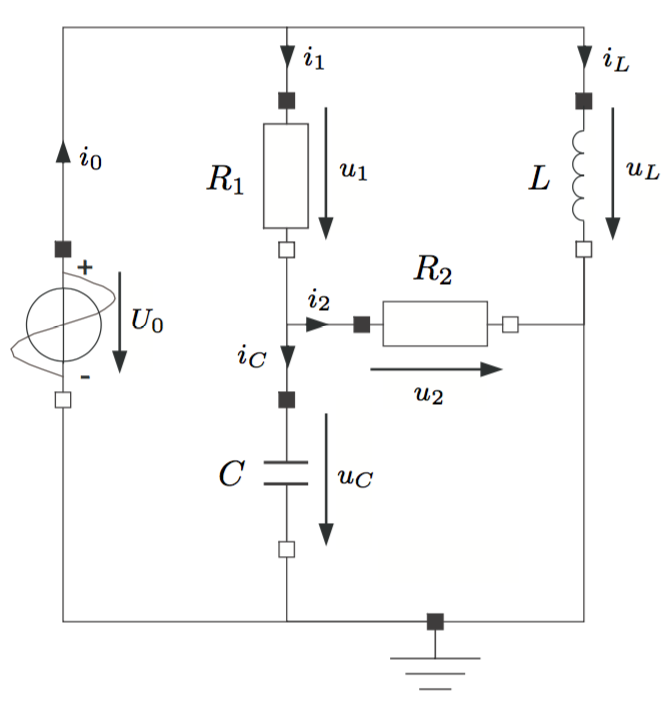
\includegraphics[width=0.5\textwidth]{graphics/rlc.png}
  \caption{RLC}
  \label{fig:RLC}
\end{figure}

Dado que en el circuito hay cinco elementos, y cada uno define dos
variables, denominadas la tensión y la intensidad de corriente a través
de dicho elemento, necesitamos diez ecuaciones para describir el modelo,
p. ej. las cinco ecuaciones correspondientes a cada elemento, las
cuales definen la relación entre la tensión y la intensidad de corriente
a través del elemento, más tres ecuaciones de malla en el voltaje
de malla, más dos ecuaciones de nodos en la corriente del nodo. Un
posible conjunto de ecuaciones es el siguiente:

\begin{eqnarray*}
u_{0} & = & \sin\left(t\right)\\
u_{1} & = & R_{1}i_{1}\\
u_{2} & = & R_{2}i_{2}\\
u_{L} & = & L\frac{du_{C}}{dt}\\
i_{C} & = & C\frac{du_{C}}{dt}\\
u_{0} & = & u_{1}+u_{2}\\
u_{L} & = & u_{1}+u_{2}\\
u_{C} & = & u_{2}\\
i_{0} & = & i_{1}+i_{L}\\
i_{1} & = & i_{2}+i_{C}
\end{eqnarray*}


El modelo Modelica correspondiente a este sistema de ecuaciones se
puede ver a continuación.

\begin{lstlisting}[language=Modelica]
  model RLC
    Real u2;
    Real u1;
    Real uL;
    Real iC;
    Real i2;
    Real u0;
    Real i0;
    Real i1;
    Real iL;
    Real uC;
    parameter Real R1;
    parameter Real R2;
    parameter Real L;
    parameter Real C;
    equation
      u0 = sin(time);
      u1 = R1 * i1;
      u2 = R2 * i2;
      uL = L * der(iL);
      iC = C *der(uC);
      u0 = u1 + uC;
      uL = u1 + u2;
      uC = u2;
      i0 = i1 + iL;
      i1 = i2 + iC;
  end RLC;
\end{lstlisting}

Al ejecutar el causalizador sobre el modelo obtenemos un nuevo modelo
cuyas ecuaciones se encuentran ordenadas vertical y horizontalmente.
El modelo resultante se puede ver a continuación.

\begin{lstlisting}[language=Modelica]
  model RLC
    Real u2;
    Real u1;
    Real uL;
    Real iC;
    Real i2;
    Real u0;
    Real i0;
    Real i1;
    Real iL;
    Real uC;
    parameter Real R1;
    parameter Real R2;
    parameter Real L;
    parameter Real C;
    equation
      u0 = sin(time);
      u2 = uC;
      u1 = (-uC)+u0;
      i2 = u2*(1/(R2));
      i1 = (1/(R1))*u1;
      iC = (-i2)+i1;
      uL = u1+u2;
      der(uC) = iC*(1/(C));
      der(iL) = (1/(L))*uL;
      i0 = i1+iL;
  end RLC; 
\end{lstlisting}

En el modelo resultante las ecuaciones están formadas por incógnitas
del lado izquierdo y por expresiones formadas por variables conocidas
del lado derecho.


\section{Circuito RLC con lazo algebraico}

Si sustituimos el capacitor del ejemplo anterior por otra resistencia
obtenemos el diagrama que se ve en la siguiente imagen.

\begin{figure}[h]
  \centering
  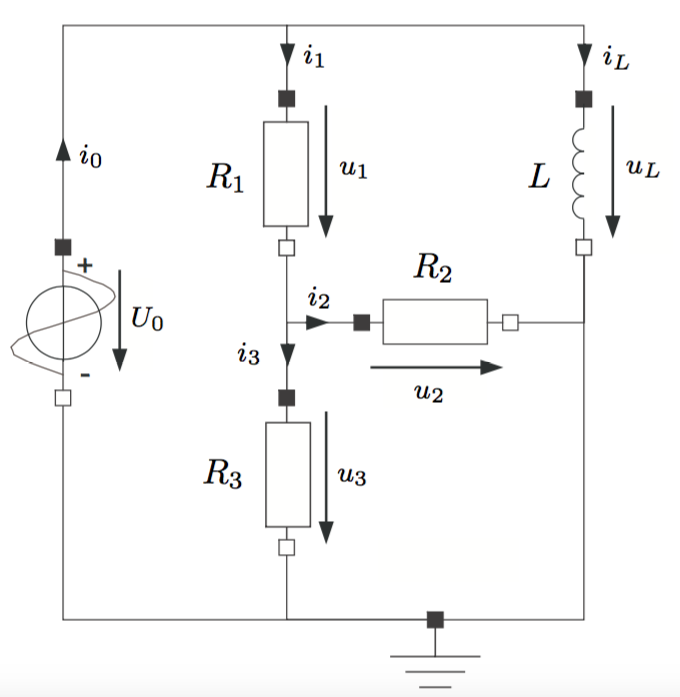
\includegraphics[width=0.5\textwidth]{graphics/rlc_loop.png}
  \caption{RLC con bucle}
  \label{fig:RLC_Loop}
\end{figure}

El sistema de ecuaciones que modela el comportamiento del circuito
es el siguiente.

\begin{eqnarray}
u_{0} & = & \sin\left(t\right)\\
u_{1} & = & R_{1}i_{1}\\
u_{2} & = & R_{2}i_{2}\\
u_{3} & = & R_{3}i_{3}\\
u_{L} & = & L\frac{di_{L}}{dt}\\
u_{0} & = & u_{1}+u_{3}\\
u_{L} & = & u_{1}+u_{2}\\
u_{3} & = & u_{2}\\
i_{0} & = & i_{1}+i_{L}\\
i_{1} & = & i_{2}+i_{3}
\end{eqnarray}


Este modelo posee un lazo algebraico, es decir un conjunto de ecuaciones
mutuamente dependientes. Para ver fácilmente el bucle algebraico,
mostramos el grafo asociado al sistema de ecuaciones. Los nodos de
las ecuaciones e incógnitas pertenecientes al bucle aparecen destacados
con un fondo gris.

\begin{figure}[h]
  \centering
  \includegraphics[width=0.5\textwidth]{graphics/rlc_loop_graph.png}
  \caption{Grafo circuito RLC}
  \label{fig:RLC}
\end{figure}

La traducción a Modelica de las ecuaciones que describen el circuito
RLC queda como se puede apreciar a continuación.

\begin{lstlisting}[language=Modelica]
  model RLC
    Real u2;
    Real u1;
    Real u3
    Real uL;
    Real u0;
    Real i0;
    Real i1;
    Real i2;
    Real i3;
    Real iL;
    parameter Real R1;
    parameter Real R2;
    parameter Real L;
    equation
      u0 = sin(time);
      u1 = R1 * i1;
      u2 = R2 * i2;
      u3 = R3 * i3; 
      uL = L * der(iL); 
      u0 = u1 + u3; 
      uL = u1 + u2;
      u3 = u2;
      i0 = i1 + iL;
      i1 = i2 + i3;
  end RLC;
\end{lstlisting}

Al ejecutar el causalizador sobre el modelo obtenemos un nuevo modelo,
cuyas ecuaciones se encuentran reordenadas de la siguiente manera.

\begin{lstlisting}[language=Modelica]
  model RLC
    Real u2;
    Real u1;
    Real u3
    Real uL;
    Real u0;
    Real i0;
    Real i1;
    Real i2;
    Real i3;
    Real iL;
    parameter Real R1;
    parameter Real R2;
    parameter Real R3;
    parameter Real L;
    equation
    u0 = sin(time);
    i1 = (1/(R1*R2+R1*R3+R2*R3))*(u0*R3+u0*R2);
    u2 = u0*(1/(R1*R2+R1*R3+R2*R3))*R2*R3;
    i3 = u0*(1/(R1*R2+R1*R3+R2*R3))*R2;
    u1 = (1/(R1*R2+R1*R3+R2*R3))*(u0*R1*R2+u0*R1*R3);
    u3 = u0*(1/(R1*R2+R1*R3+R2*R3))*R2*R3;
    i2 = u0*(1/(R1*R2+R1*R3+R2*R3))*R3;
    uL = u1+u2;
    der(iL) = (1/(L))*uL;
    i0 = i1+iL;
  end RLC;
\end{lstlisting}

Al igual que con el caso de la sección anterior, el modelo resultante
se encuentra ordenado vertical y horizontalmente. En este caso el
bucle pudo ser resuelto (todos los lados derechos de las ecuaciones
dependen solo de la variable $u_{0}$) porque las ecuaciones que lo
conformaban eran lineales. Si ese no hubiese sido el caso lo que hubiésemos
obtenido es un sistema ordenado donde el bucle se sustituye por una
función externa como la que se ve a continuación.

\begin{lstlisting}
(u0,i1,u2,i3,u1,u3,i2) = fsolve(u0);
\end{lstlisting}

Esta función externa resuelve el sistema de ecuaciones formado por
las ecuaciones del bucle mediante métodos de integración numérica.


\chapter{\label{chap:Prueba-de-eficiencia}Prueba de eficiencia}

En la sección \ref{sub:Optimizaci=0000F3n} se presentó un algoritmo
simple el cual permite optimizar el proceso de causalización. En esta
sección vamos a comparar, utilizando un ejemplo, los tiempos de ejecución
del proceso de causalización completo con los tiempos del proceso
de causalización sin la optimización (es decir utilizando solo el
algoritmo de Tarjan). El objetivo es evidenciar empíricamente la ganancia
que se obtuvo al incluir el algoritmo simple al proceso de causalización.

Para medir los tiempos de ejecución de las diferentes estrategias
armamos un test, el cual recibe como entrada un modelo Modelica y
lo causaliza utilizando las tres estrategias anteriormente mencionadas.
Al finalizar imprime el tiempo que demoro en ejecutarse cada estrategia.
El test se encuentra implementado en el archivo test/causalize/performance\_test.cpp.


\section{Primer caso}

Para realizar las puebas de eficiencia elegimos un modelo que representa
al fenómino de transmisión de masa/energía en una dimensión. Este
sistema resulta apropiado para la prueba de eficiencia porque, como
vamos a ver cuando presentemos el modelos Modelica, podemos controlar
el tamaño del mismo modificando un solo parámetro.

La ecuación que representa este fenómeno es la siguiente:

\begin{center}
$\frac{\partial u(x,t)}{\partial t}+a\frac{\partial u(x,t)}{\partial x}=d\frac{\partial^{2}u(x,t)}{\partial x^{2}}$
\par\end{center}

donde $u(x,t)$ representa la concentración de masa o energía en la
coordenada espacial $x$ en el tiempo $t$. 

La ecuación presenta derivadas en función de la componente espacial,
lo que la transforma en una ecuación en derivadas parciales. Ésta
es convertida en una ecuación diferencial ordinaria utilizando el
Método de Líneas \citep{CK06} el cual discretiza la componente espacial
usando diferencias finitas en $N$ segmentos. Cuanto mayor sea $N$
mejor será la aproximación. Una vez discretizada la componente espacial
obtenemos el siguiente conjunto de ODEs:

\begin{eqnarray*}
\dot{u}_{n}(t) & = & 0\\
\dot{u}_{1}(t) & = & \frac{u_{1}(t)-u_{2}(t)}{\frac{1}{N}}\\
\dot{u}_{i}(t) & = & \frac{u_{i+1}(t)-u_{i}(t)}{\frac{1}{N}}+\frac{u_{i-1}(t)-u_{i}(t)}{\frac{\gamma}{N}}\;
\end{eqnarray*}


para $i\epsilon[2:N-1]$.

El modelo Modelica correspondiente tiene la siguiente forma.

\begin{lstlisting}[language=Modelica]
  model OneDHeatTransferTI_FD
    parameter Real L = 0.2;
    constant Integer N = 100;
    parameter Real T0 = 273.15;
    parameter Real TN = 330;
    parameter Real cp = 910;
    parameter Real lambda = 237;
    parameter Real rho = 2712;
    final parameter
    Real dx = L / (N - 1);
    Real T[N] ;
    initial algorithm
      for i in 1:N - 1 loop
        T[i] := T0;
      end for;
      T[N] := TN;
    equation
      der(T[N]) = 0;
      for i in 2:N - 1 loop
        der(T[i]) = lambda * ((T[i + 1] - T[i]) / dx + ((-T[i]) + T[i - 1]) / dx) / cp / rho / dx;
      end for;
      der(T[1]) = lambda * ((T[2] - T[1]) / dx) / cp / rho / dx;
  end OneDHeatTransferTI_FD; 
\end{lstlisting}

Al ejecutar el test de performance sobre el modelo obtenemos una salida
como la que siguiente:

\begin{figure}[H]
  \centering
  \verb+Simple strategy: 0.020906 Tarjan strategy: 0.021469 Full Causalization strategy: 0.020833+
\end{figure}

donde cada estrategia reporta (en segundos) el tiempo utilizado.

En el gráfico \ref{fig:OneDHeatTransfer} se puede ver el resultado
de aplicar el test sobre modelos \verb+OneDHeatTransferTI_FD+ con
diferentes tamaños de la constante \verb+N+.

\begin{figure}[h]
  \centering
  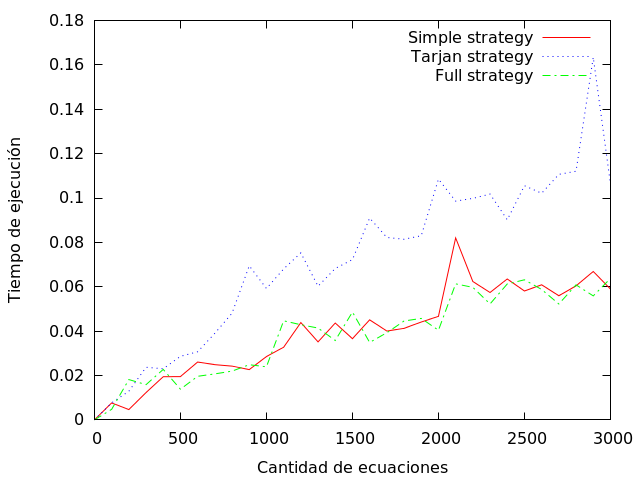
\includegraphics[width=0.8\textwidth]{graphics/revision/OneDHeatTransfer.png}
  \caption{OneDHeatTransfer}
  \label{fig:OneDHeatTransfer}
\end{figure}

Según los calculos realizados en la sección \ref{sub:ComplejidadTarjan1}
la complejidad de la estrategia compleja es $O(V^{2})$. En el caso
de la estrategía simple (ver sección \ref{sub:Optimizaci=0000F3n}),
la complejidad temporal es $O(V+V\times\log V)$. En el gráfico \ref{fig:OneDHeatTransfer}
se puede apreciar que el crecimiento del tiempo de ejecución en función
de la cantidad de ecuaciones del sistema se condice con los valores
de complejidad calculados. Respecto a la estrategía completa de causalización,
lo que se puede ver en el gráfico es que la curva es similar a la
de la estrategía simple. Esto es porque el modelo de ejemplo no posee
lazos algebraicos y por lo tanto solo es necesario la aplicación de
la estrategía simple.


\section{Segundo caso}

Para analizar qué sucede con la estrategía completa en el caso en
el que el modelo sí posee lazos algebraicos lo que hicimos fue agregar
un lazo al ejemplo \verb+OneDHeatTransferTI_FD+. La modificación
consistió en agregar el arreglo \verb+U+ junto con un conjunto de
ecuaciones todas incluidas en un bucle algebraico. A continuación
se puede ver el modelo modificado.

\begin{lstlisting}[language=Modelica]
  model OneDHeatTransferTI_FD
    parameter Real L = 0.2;
    constant Integer N = 100;
    parameter Real T0 = 273.15;
    parameter Real TN = 330;
    parameter Real cp = 910;
    parameter Real lambda = 237;
    parameter Real rho = 2712;
    final parameter
    Real dx = L / (N - 1);
    Real T[N];
    Real U[N]; 
    initial algorithm
      for i in 1:N - 1 loop
        T[i] := T0;
      end for;
      T[N] := TN;
    equation
      der(T[N]) = 0;
      U[1]*U[2]=0;
      for i in 2:N - 1 loop
        der(T[i]) = der(T[i-1]) + lambda * ((T[i + 1] - T[i]) / dx + ((-T[i]) + T[i - 1]) / dx) / cp / rho / dx;
        U[i] = U[i+1]+U[i-1]; 
      end for;
      der(T[1]) = lambda * ((T[2] - T[1]) / dx) / cp / rho / dx;
      U[N] = U[N-1]*2+sin(U[N]); 
  end OneDHeatTransferTI_FD; 
\end{lstlisting}

Al ejecutar el test sobre este nuevo modelo, para los mismos valores
de la constante \verb+N+, obtenemos el gráfico \ref{fig:OneDHeatTransfer_loop}.

\begin{figure}[h]
  \centering
  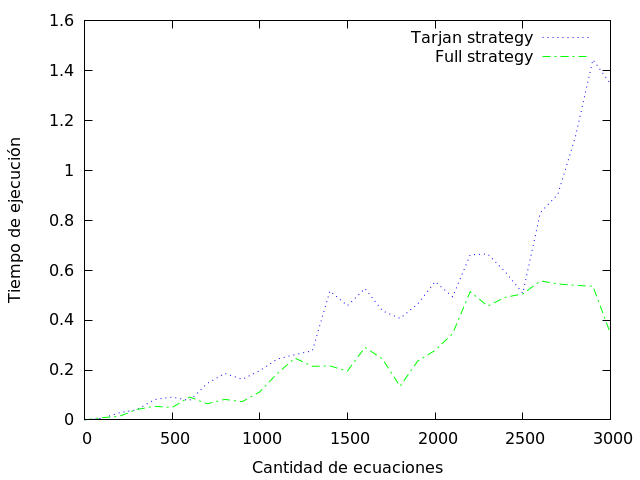
\includegraphics[width=0.8\textwidth]{graphics/revision/OneDHeatTransfer_loop.png}
  \caption{OneDHeatTransfer con bucle algebraico}
  \label{fig:OneDHeatTransfer_loop}
\end{figure}

La línea punteada representa los tiempos de ejecución resultantes
de aplicar solo el algoritmo de Tarjan. La línea semi-punteada representa
los tiempos de ejecución de la estrategía de causalización completa,
es decir ejecutando el algoritmo simple antes de aplicar Tarjan. La
línea continua grafica los tiempos de la estrategía simple. Dada la
existencia del bucle algebraico el algoritmo simple no termina por
lo tanto no tiene sentido incluirlo (de manera aislada) en la comparación.
La diferencia de crecimiento entre las curvas que representan la aplicación
de Tarjan y la aplicación de la estrategía completa se condice con
los resultados obtenidos en la sección \ref{sub:Optimizaci=0000F3n}
y permite ver más claramente cómo la inclusión del algoritmo simple
constituye una optimización del proceso de causalización.


\chapter{\label{chap:Conclusiones}Conclusiones}


\section{Conclusiones generales}

En este trabajo se presentó la implementación en C++ de la etapa de
causalización de ecuaciones de un compilador Modelica. El trabajo
estuvo enmarcado dentro del proyecto de investigación “Modelado, Simulación
y Control en Tiempo Real con Aplicaciones en Electrónica de Potencia”
de la Universidad Nacional de Rosario. Uno de los objectivos de dicho
proyecto es el desarrollo de un compilador Modelica, denominado ModelicaCC
(Modelica C Compiler), a partir del cual poder investigar distintos
algoritmos en relación a modelos de gran escala. Puntualmente, la
implementación aquí presentada de la etapa de causalización constituye
el puntapié inicial para la implementación de un algoritmo de causalización
vectorial, es decir, un algoritmo que realice la causalización de
ecuaciones sin la necesidad de expandir los arreglos ni las estructuras
repetitivas (como por ejmplo las For-Equation) presentes en el modelo.
Dicha implementación se puede ver en el siguiente artículo \citep{lsmodelica}.

\begin{comment}
En la primer parte del trabajo se introdujo el lenguaje Modelica,
así como también se introdujeron las nociones de ecuacion diferencial
ordinaria y ecuación diferencial algebraica. Se planteó la necesidad
de incluir en el proceso de compilación de un modelo Modelica, un
componente capaz de transformar los modelos representados por ecuaciones
diferenciales algebraicas en modelos equivalentes representados por
ecuaciones diferenciales ordinarias. Esta necesidad surge a partir
de el hecho de que la mayoría de los integradores númericos, necesarios
para la simulación de un modelo Modelica, esperan modelos respresentados
mediante eucaciones diferenciales ordinarias. También presentamos
el algoritmo de Tarjan como el más adecuado para resolver la tarea
de causalizaión de ecuaciones, es decir la transformación de ecuaciones
diferenciales algebraicas en ecuaciones diferenciales ordinarias.
Por último introdujimos el compilador \textit{ModelicaCC}, su arquitectura
general y los diferentes componentes que implementan cada una de las
etapas de compilación.
\end{comment}


Estudiamos e implementamos tres estrategias distintas para resolver
el problema de causalización analizando la complejidad computacional
de cada una de ellas. La aplicación del algoritmo de Tarjan conlleva
el cálculo de un enparejamiento sobre el grafo lo cual tiene un costo
cuadrático con respecto a los vértices. Basándonos en una versión
simplificada del algoritmo de Tarjan introdujimos una nueva formulación
del algorítmo (Sección \ref{sub:Optimizaci=0000F3n}) que permite
llevar a cabo la causalización en tiempo logarítmico cuando el modelo
no presenta lazos algebraicos. Este algoritmo resultó una optimización
en todos los casos, ya que para los modelos que sí presentan bucles
algebraicos, el algoritmo reduce el tamaño del grafo eliminando (y
causalizando) los vértices que no pertenecen a algún bucle, para luego
aplicar el algoritmo de Tarjan calculando el emparejamiento sobre
un grafo más pequeño.

La implementación de las estrategías de causalización se realizó utilizando
librerías abiertas como la biblioteca Boost Graph utilizada para la
implementación del algoritmo de Tarjan, así como también para la representacion
de los grafos y la biblioteca GiNaC para manipulación simbólica. 

En el capítulo \ref{chap:Ejemplos} presentamos dos ejemplos del campo
eléctrico demostrando que el algoritmo produce un resultado correcto
tanto ante la presencia o ausencia de lazos algebraicos.

Luego en el capítulo \ref{chap:Prueba-de-eficiencia} se presentó
un ejemplo que permite ver más claramente de qué manera la inclusión
del algoritmo simple resulta en una optimización del proceso de causalización. 

Por último, en el apéndice se incluyó el detalle de los tests unitarios
escritos para validar los diferentes componentes desarrollados durante
esta tesina.


\section{Trabajo a futuro}

Algunos puntos quedan como trabajo a futuro de esta tesina:
\begin{itemize}
\item Singularidades estructurales: La transformación de ecuaciones diferenciales
algebráicas en ecuaciones diferenciales ordinarias no siempre puede
ser llevada a cabo utilizando los algoritmos presentados en este trabajo.
Ciertos modelos presentan lo que se conoce como ``singularidad estructural''
lo que llevará al algoritmo de Tarjan (o sus variantes) a fallar debido
a que algunos nodos quedan desconectados. En este caso debe ser aplicado
previamente el algoritmo de Pantelides \citep{Pan88} para transformar
al sistema en uno que sí se pueda causalizar.
\item Otro punto a tratar es la resolución de lazos algebraicos. Los algoritmos
aquí presentados se encargan de detectar e identificar las variables
y ecuaciones que deben ser resueltas en conjunto pero este lazo puede
ser de gran tamaño. Una opción para reducir el tamaño del lazo es
aplicar la técnica conocida como Tearing \citep{CK06} la cual considera
conocida una variable del lazo y trata de despejar las otras a partir
de ésta. En la presente implementación esta técnica no es utilizado
por lo cual los lazo algebraicos quedan del tamaño con el cual son
identificados.
\item Causalización de ecuaciones for sin expansión: En esta versión del
causalizador de ecuaciones las estructuras repetitivas como las ecuaciones
for se expanden. Esta solución no es eficiente para modelo de gran
escala. En \citep{lsmodelica} se plantea una versión vectorial del
algoritmo de Tarjan la cual permite realizar la causalización de ecuaciones
sin la necesidad de expandir las estructuras repetitivas. La implementación
de dicho algoritmo vectorial queda pendiente para futuras versiones
del causalizador.
\end{itemize}
\appendix

\chapter{\label{sec:Tests-unitarios}Tests unitarios}

Los tests unitarios se desarrollaron utilizando la biblioteca Boost
Test \citep{ROTEST}. Para cada componente que deseábamos testear
escribimos un archivo diferente. Cada archivo se compone de un conjunto
de funciones denotando cada una un unit test más una función que provee
la biblioteca Boost Test, \verb+init_unit_test_suite+, en la cual
se listan los tests a ejecutar. Estos archivos luego se compilan en
ejecutables. Al ejecutarlos se ejecutan los tests listados en la función
\verb+init_unit_test_suite+. Las aserciones las realizamos utilizando
la función \verb+BOOST_CHECK+. A modo ilustrativo vamos a ver una
parte del archivo apply\_Tarjan\_test.cpp que corresponde al unit
test de la función \verb+apply_Tarjan+.

\begin{lstlisting}
#include <boost/test/unit_test.hpp>
#include <boost/test/included/unit_test.hpp>
#include <causalize/apply_Tarjan.h>

using namespace boost::unit_test;

void apply_Tarjan_test() {
   ...
   BOOST_CHECK(apply_Tarjan(graph, components) == 4);
}

test_suite* init_unit_test_suite( int, char* [] ) {
    framework::master_test_suite().p_name.value = "Apply Tarjan";
    framework::master_test_suite().add( BOOST_TEST_CASE( &apply_Tarjan_test ));
    return 0;
}
\end{lstlisting}

En esta porción de código podemos ver la función \verb+apply_Tarjan_test()+
la cual constituye el unit test. También podemos ver la declaración
de la función donde se agrega el test \verb+apply_Tarjan_test+ al
test suite. Al ejecutar el test la salida es la siguiente:

\begin{verbatim}
    $ ./apply_Tarjan_test
    Running 1 test case...

    *** No errors detected 
\end{verbatim}

Escribimos unit tests para los siguientes componentes:
\begin{itemize}
\item La función process\_for\_equations (ver \ref{sub:Expansi=0000F3n-de-ecuaciones}).
\item La función apply\_Tarjan (ver \ref{sub:Aplicaci=0000F3n-Tarjan-Boost}).
\item La clase Causalization Strategy (ver \ref{sub:Optimizaci=0000F3n}).
\end{itemize}
A continuación vamos a describir cada uno de los unit tests.


\section{process\_for\_equation\_test}

Para probar la expansión de ecuaciones de tipo For-Equation decidimos
armar diferentes modelos Modelica, cada uno capturando alguna de las
alternativas que existen para escribir este tipo de ecuaciones. Luego
escribimos un test unitario para cada uno de estos modelos. Los test
verifican que la cantidad de ecuaciones generadas coincida con lo
que se definió en el \verb+for_index+ (ver sección \ref{sub:Expansi=0000F3n-de-ecuaciones})
y que la instanciación y evaluación de cada ecuación sea la correcta.

Los diferentes modelos se pueden ver a continuación.

\begin{figure}[H]
  \begin{subfigure}[b]{0.5\textwidth}
	  \begin{lstlisting}[language=Modelica]
	    model ForExample
	      Real a[10];
	    equation
	      for i in 1:10 loop
	        a[i] = i;
	      end for;
	    end ForExample;
	  \end{lstlisting}
	  \subcaption{\label{fig:for_model_1}}
  \end{subfigure}
  \begin{subfigure}[b]{0.5\textwidth}
	  \begin{lstlisting}[language=Modelica]
	    model ForExample
	      constant Integer N = 11;
	      constant Integer S = 1;
	      constant Integer M = 20;
	      Real a[10];
	    equation
	      for i in N:S:M loop
	        a[i] = i;
	      end for;
	    end ForExample;
	  \end{lstlisting}
      \subcaption{\label{fig:for_model_2}}
  \end{subfigure}
  \begin{subfigure}[b]{0.5\textwidth}
	  \begin{lstlisting}[language=Modelica]
	    model ForExample
	      Real a[10];
	    equation
	      for i in {1,2,3,4,5} loop 
	          a[i] = i; 
	      end for;
	    end ForExample;
	  \end{lstlisting}
  	\subcaption{\label{fig:for_model_3}}
  \end{subfigure}
  \begin{subfigure}[b]{0.5\textwidth}
	  \begin{lstlisting}[language=Modelica]
	    model ForExample
	      Real a[10];
	    equation
	      for i in 1:10 loop
	          a[i+1] = i+1; 
	      end for;
	    end ForExample;
	  \end{lstlisting}
  	\subcaption{\label{fig:for_model_4}}
  \end{subfigure}
\end{figure}

Los primeros tres modelos permiten verificar el procesamiento del
\verb+for_index+ en sus diferentes variantes. El cuarto modelo permite
verificar la evaluación de las expresiones resultantes de la instanciación
del índice de iteración. En todos los modelos se verifica que la cantidad
de ecuaciones generadas y la instanciación del índice en cada una
sea la correcta.

A continuación vemos el código del unit test para el primer caso de
prueba. Los otros tests, muy similares al que mostramos acá, se pueden
encontrar en el archivo test/causalize/for\_unrolling/process\_for\_equations\_test.cpp.

\begin{lstlisting}
  void unrolling_test_1() {
   bool r;
    StoredDef sd=parseFile("for_example_1.mo",r);
    if (!r) {
      cout << "Couldn't open for_example.mo file" << endl;
      return;
    }
    Class ast_c = boost::get<Class>(sd.classes().front());
    MMO_Class c(ast_c); 
    int equationsBefore = c.equations().equations().size(); 
    Causalize::process_for_equations(c);
    int equationsAfter = c.equations().equations().size();
    BOOST_CHECK(equationsAfter == 10);
    int i=1;
    foreach_(Equation eq, c.equations().equations()) {
      BOOST_CHECK(is<Equality>(eq));
      Equality eqEq = get<Equality>(eq);
      Expression expLeft = eqEq.left();
      BOOST_CHECK(is<Reference>(expLeft));
      Reference array = get<Reference>(expLeft);
      BOOST_CHECK(array.ref().size() == 1);
      ExpList indexes = get<1>(array.ref().front());
      BOOST_CHECK(indexes.size() == 1);
      Expression index = indexes.front();
      BOOST_CHECK((int)get<Modelica::AST::Integer>(index) == i);
      Expression expRight = eqEq.right();
      is<Integer>(expRight);
      BOOST_CHECK(get<Integer>(expRight) == i);
      i++;
    }
  }
\end{lstlisting}

La primer aserción que aparece en el test es la que verfica que la
cantidad de ecuaciones generadas sea la correcta, en nuestro caso
el número correcto es 10. Luego se verifica que cada ecuación se haya
generado correctamente. Primero se revisa que la variable del lado
izquierdo de cada ecuación sea un arreglo unidimensional y que la
instanciación del índice del arreglo sea la correcta. Luego se verifica
que la expresión del lado derecho sea de tipo entero y que la instanciación
y evaluación (en este caso trivial) de la misma sea que corresponde.


\section{apply\_Tarjan\_test}

Para realizar el test de la función \verb+apply_Tarjan+, descripta
en la sección \ref{sub:Aplicaci=0000F3n-Tarjan-Boost}, construimos
un grafo de causalización sencillo, al cual le ``fabricamos'' un
bucle. El grafo que creamos es un grafo con 10 vértices y 11 aristas.
La declaración del grafo se puede ver a continuación:

\begin{lstlisting}
  CausalizationGraph graph;
  VertexProperties vp1;
  vp1.type = E;
  Vertex e1 = add_vertex(vp1, graph);
  VertexProperties vp2;
  vp2.type = U;
  Vertex u1 = add_vertex(vp2, graph);
  VertexProperties vp3;
  vp3.type = E;
  Vertex e2 = add_vertex(vp3, graph);
  VertexProperties vp4;
  vp4.type = U;
  Vertex u2 = add_vertex(vp4, graph);
  VertexProperties vp5;
  vp5.type = E;
  Vertex e3 = add_vertex(vp5, graph);
  VertexProperties vp6;
  vp6.type = U;
  Vertex u3 = add_vertex(vp6, graph);
  VertexProperties vp7;
  vp7.type = E;
  Vertex e4 = add_vertex(vp7, graph);
  VertexProperties vp8;
  vp8.type = U;
  Vertex u4 = add_vertex(vp8, graph);
  VertexProperties vp9;
  vp9.type = E;
  Vertex e5 = add_vertex(vp9, graph);
  VertexProperties vp10;
  vp10.type = U;
  Vertex u5 = add_vertex(vp10, graph);
  add_edge(e1, u3, graph);
  add_edge(e1, u4, graph);
  add_edge(e2, u2, graph);
  add_edge(e3, u2, graph);
  add_edge(e4, u1, graph);
  add_edge(e4, u2, graph);
  add_edge(e5, u1, graph);
  // The following edges  form a cycle.
  add_edge(e3, u3, graph);
  add_edge(e3, u5, graph);
  add_edge(e5, u3, graph);
  add_edge(e5, u5, graph);
\end{lstlisting}

Las últimas 4 aristas forman el único bucle del grafo.

El algoritmo de Tarjan se aplica sobre un grafo dirigido que resulta
de aplicar los pasos descriptos en \ref{sub:Aplicaci=0000F3n-Tarjan-Boost}
a un grafo no dirigido. Para el caso del grafo utilizado en este test
el grafo dirigido resultante es un grafo de 5 vértices con un bucle.
Por lo tanto el algoritmo de Tarjan debe encontrar 4 componentes fuertemente
conexos. Esta aserción es la que utilizamos para probar nuestra función
\verb+apply_Tarjan+ y lo hacemos de la siguiente manera:



\begin{lstlisting}
  std::map<int, causalize::Component> components;
  BOOST_CHECK(apply_Tarjan(graph, components) == 4);
\end{lstlisting}


\section{causalization\_strategy\_test}

Este es el test asociado a la clase \verb+CausalizationStrategy+
(ver capítulo \ref{chap:Implementaci=0000F3n-etapa-de}). El mismo
permite validar que el modelo resultante de aplicar el método \verb+CausalizationStrategy::causalize+
es un modelo causal. Para validar la causalidad de un modelo escibimos
la función \verb+check_causality+ la cual se puede encontrar en el
archivo test/causalize/causalization\_strategy\_test.cpp. La función
recibe como parámetros el modelo a validar y la lista de incógnitas
de dicho modelo. La validación se realiza ecuación por ecuación, verificando
para cada una que la incógnita del lado izquierda pueda ser calculada
a partir de las variables que aparecen del lado derecho. Dicho de
otra manera lo que verificamos es que las variables que aparecen del
lado derecho de cada ecuación sean variables conocidas (porque ya
fueron calculadas por una ecuación anterior). El código de la función
se puede ver a continuación.

\begin{lstlisting}
  void check_causality(MMO_Class &mmoClass, ExpList unknowns) {
  const EquationList &causalEqs = mmoClass.equations_ref().equations_ref();
  ExpList knowns;
  foreach_(Equation equation, causalEqs) {
    Equality eqEq = boost::get<Equality>(equation);
    foreach_(Expression unknown, unknowns) {
      Modelica::contains occurrs(unknown);
      if (boost::apply_visitor(occurrs, eqEq.right_ref())) {
        bool isKnown = false;
        foreach_(Expression known, knowns) {
          if(known == unknown) {
            isKnown = true;
          }
        }
        BOOST_CHECK(isKnown);
      }
    }
    Expression leftExpression = eqEq.left_ref();
    if (is<Reference>(leftExpression)) {
      knowns.push_back(leftExpression);
    } else if (is<Call>(leftExpression)) {
      Call call = boost::get<Call>(leftExpression);
      if (call.name()=="der")
        knowns.push_back(leftExpression);
    } else if (is<Output>(leftExpression)) {
      Output output = boost::get<Output>(leftExpression);
      foreach_(OptExp oe, output.args()) {
        if (oe)
          knowns.push_back(oe.get());
      }
    } else {
      ERROR("Unexpected type for equation's left expression\n");
    }
  }
}
\end{lstlisting}

La función declara una lista de variables conocidas. Luego itera sobre
las ecuaciones del modelo que recibe como parámetro. Lo primero que
hacemos para cada ecuación es validar que las variables que aparecen
en el lado derecho de la ecuación se encuentren en la lista de variables
conocidas. Esta lista se popula con las variables que aparecen en
lado izquierdo de cada ecuación. Si el test se ejecuta satisfactoriamente
es porque para cada ecuación, evaluada en el orden en el que se encuentra
definida en el modelo, las variables del lado derecho son todas variables
conocidas y de esta manera es posible resolver la ecuación y obtener
el valor de la variable que se encuentra en el lado izquierdo.

Los casos de prueba que utilizamos fueron los presentados en el capítulo
\ref{chap:Ejemplos}.

\bibliographystyle{plainnat}
\bibliography{bibliography}

\end{document}
